\documentclass[usenames,dvipsnames]{article}
\usepackage[dvipsnames]{xcolor}
\usepackage{graphicx} % Required for inserting images
\usepackage{float} % For exact placement of tutorial figures



\usepackage{bm}
\usepackage{frcursive}
\usepackage{xfrac}
\usepackage{mathrsfs}
\usepackage{mathtools}

\usepackage{fancyvrb}
\usepackage{xspace}
\usepackage{amsmath}
\usepackage{amssymb}
\usepackage{amsthm}


%\usepackage{xcolor}
\usepackage{minted}



\usepackage{hyperref}
\usepackage{tikz}
\usetikzlibrary{arrows, fit, positioning, shapes, calc, backgrounds}





\title{Diffusion and flow matching tutorial: How we generate images, video, speech and protein structures}
\author{Nando de Freitas and Everyone}
\date{\today}

\DeclarePairedDelimiter{\norm}{\lVert}{\rVert}

\newcommand{\myvec}[1]{\mathbf{#1}}
\newcommand{\myvecsym}[1]{\boldsymbol{#1}}
\newcommand{\mytensor}[1]{\mathbf{\tilde{#1}}}

\newcommand{\vk}{\myvec{\textcolor{SeaGreen}{k}}}
\newcommand{\rvk}{\myvec{\textcolor{SeaGreen}{k}}}

\newcommand{\vx}{\myvec{\textcolor{ForestGreen}{x}}}
\newcommand{\rvx}{\myvec{\textcolor{ForestGreen}{x}}}
\newcommand{\vz}{\myvec{\textcolor{Red}{z}}}
\newcommand{\vh}{\myvec{\textcolor{Cyan}{h}}}
\newcommand{\vc}{\myvec{\textcolor{purple}{c}}}
\newcommand{\rvz}{\myvec{\textcolor{Red}{z}}}
\newcommand{\vy}{\myvec{\textcolor{Magenta}{y}}}
\newcommand{\rvy}{\myvec{\textcolor{Magenta}{y}}}
\newcommand{\vs}{\myvec{\textcolor{Cyan}{s}}}
\newcommand{\rvs}{\myvec{\textcolor{Cyan}{s}}}
\newcommand{\vu}{\myvec{\textcolor{orange}{u}}}
\newcommand{\vv}{\myvec{\textcolor{Cyan}{v}}}
\newcommand{\rvv}{\myvec{\textcolor{Cyan}{v}}}


\newcommand{\vzero}{\myvec{\textcolor{olive}{0}}}
\newcommand{\vI}{\myvec{\textcolor{olive}{I}}}

%\newcommand{\vtheta}{\myvec{\vtheta}}
\newcommand{\vvarphi}{\myvecsym{\textcolor{NavyBlue}{\varphi}}}
\newcommand{\vtheta}{\myvecsym{\textcolor{blue}{\theta}}}
\newcommand{\valpha}{\myvecsym{\textcolor{purple}{\alpha}}}
\newcommand{\vsigma}{\myvecsym{\textcolor{purple}{\sigma}}}
\newcommand{\vepsilon}{\myvecsym{\textcolor{CarnationPink}{\epsilon}}}
\newcommand{\vmu}{\myvecsym{\textcolor{teal}{\mu}}}

\newcommand{\loss}{{\cal L}}
\newcommand{\gauss}{\mathcal{N}}
\newcommand{\E}{\mathbb{E}} % \E{f(x)}
\newcommand{\pT}{p_{\vtheta}}


\newcommand{\be}{\begin{equation}}
\newcommand{\ee}{\end{equation}}
% for cormen.cls, we define
%\newcommand{\be}{\begin{eqnarray}}
%\newcommand{\ee}{\end{eqnarray}}
% NOTE that use of eqnarray causes issues with \label and \cref

\newcommand{\bea}{\begin{eqnarray}}
\newcommand{\eea}{\end{eqnarray}}
\newcommand{\beaa}{\begin{eqnarray*}}
\newcommand{\eeaa}{\end{eqnarray*}}
\newcommand{\ba}{\begin{align*}}
\newcommand{\ea}{\end{align*}}



% Macros for consistent formatting
\newcommand{\action}{\textbf{\textcolor{red}{$a$}}}
%\newcommand{\vx}{\textbf{\textcolor{ForestGreen}{$x$}}}
\newcommand{\reward}{\textbf{\textcolor{purple}{$r$}}}
\newcommand{\nextaction}{\textbf{\textcolor{red}{$a'$}}}
\newcommand{\nextobs}{\textbf{\textcolor{ForestGreen}{$o'$}}}
\newcommand{\params}{\textbf{\textcolor{blue}{$\theta$}}}
\newcommand{\return}{\textbf{\textcolor{cyan}{R}}}




\begin{document}

\maketitle




%%%%%%%%%%%%%%%%%%%%%%%%%%%%%%%%%%%%%%%%%%%%%%%%%
\section{Introduction}

Diffusion and flow matching are the standard ways for generating images, video, speech, music and even protein structures and molecular simulations. 

This tutorial aims at deriving the basic equations needed to understand these applications and the code behind them. Regardless of the modality, the code will be pretty much the same. While there are other derivations using variational methods, here we will simply use a fundamental learning principle: match imagination to reality. That is, what the model imagines, predicts, or generates, must match the real data. This is the principle used to train LLMs too, but while LLMs typically use the Maximum Likelihood principle, here we will use the Score Matching principle. 

After explaining diffusion, we will derive a simple but very powerful approach based on conditional expectation and ordinary differential equations (ODEs). This will allow us to arrive at flow matching, where very deep neural networks can be interpreted as running ODEs with transformer blocks to generate data.

To understand diffusion from first principles, we first need to derive a loss function, which will then be used to train the generative model. The loss function is often reparameterised to make it numerically stable. The data for the loss function will consist of the original image and noisy samples generated by a forward diffusion process, as shown in Figure \ref{fig:simpleDiffusion}. Using these data, we will \emph{train} a neural network to undo the process of adding noise. Finally, such a network will enable us to start with any random sample and reverse it until we get an image. We will refer to this reverse process as \emph{inference}.
\begin{figure}[h!]
\centering
\resizebox{\textwidth}{!}{%
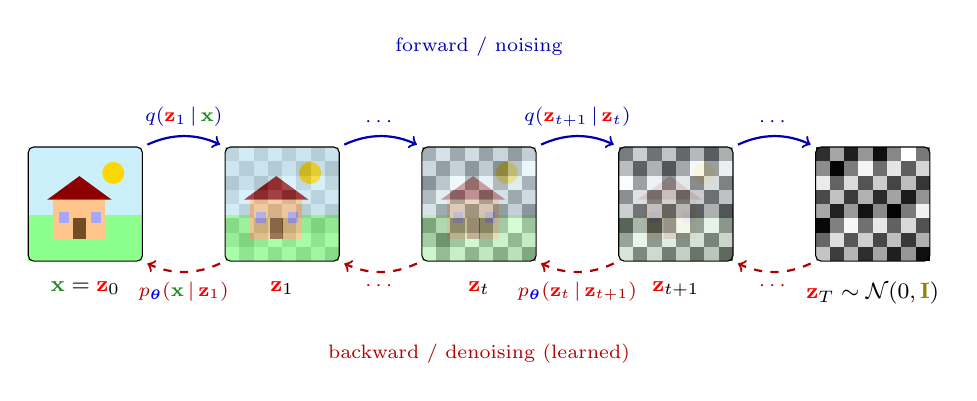
\begin{tikzpicture}[
    every node/.style={font=\small},
    fwd/.style={->, thick, blue!70!black, shorten >=2pt, shorten <=2pt},
    bwd/.style={->, thick, red!70!black, shorten >=2pt, shorten <=2pt, dashed},
    lbl/.style={font=\scriptsize, midway},
]
    % A small deterministic "image + noise" thumbnail.  The clean picture is a
    % simple sky/ground/house icon; the grey cells become more opaque as t grows.
    \newcommand{\noisythumb}[5]{%
        \node[inner sep=0pt, outer sep=0pt, minimum width=1.45cm,
              minimum height=1.45cm] (#1) at (#2,0) {};
        \begin{scope}[shift={($(#1.south west)$)}]
            \fill[white] (0,0) rectangle (1.45,1.45);
            \begin{scope}[opacity=#4]
                \fill[cyan!20] (0,0.58) rectangle (1.45,1.45);
                \fill[green!45] (0,0) rectangle (1.45,0.58);
                \fill[yellow!75!orange] (1.08,1.12) circle (0.14);
                \fill[orange!45] (0.32,0.28) rectangle (0.98,0.78);
                \fill[red!55!black] (0.24,0.78) -- (0.65,1.08) -- (1.06,0.78) -- cycle;
                \fill[brown!60!black] (0.57,0.28) rectangle (0.74,0.55);
                \fill[blue!35] (0.39,0.48) rectangle (0.52,0.62);
                \fill[blue!35] (0.80,0.48) rectangle (0.93,0.62);
            \end{scope}
            \foreach \row in {0,...,7} {
                \foreach \col in {0,...,7} {
                    \pgfmathtruncatemacro{\shade}{mod(37*\row + 53*\col + 23*#5,100)}
                    \fill[black!\shade, opacity=#5]
                        (0.18125*\col,0.18125*\row) rectangle +(0.18125,0.18125);
                }
            }
            \node[draw, rounded corners=2pt, minimum width=1.45cm,
                  minimum height=1.45cm, inner sep=0pt, fill opacity=0,
                  text opacity=1] at (0.725,0.725) {};
        \end{scope}
        \node[font=\footnotesize, below=0.14cm of #1] {#3};
    }

    \noisythumb{x}{0.0}{$\vx=\vz_0$}{1.00}{0.00}
    \noisythumb{z1}{2.5}{$\vz_1$}{0.88}{0.18}
    \noisythumb{z2}{5.0}{$\vz_t$}{0.60}{0.42}
    \noisythumb{z3}{7.5}{$\vz_{t+1}$}{0.32}{0.68}
    \noisythumb{zT}{10.0}{$\vz_T\sim\gauss(0,\vI)$}{0.00}{1.00}

    \draw[fwd] (x.north east)  to[bend left=25] node[lbl, above] {$q(\vz_1\,{|}\,\vx)$} (z1.north west);
    \draw[fwd] (z1.north east) to[bend left=25] node[lbl, above] {$\cdots$} (z2.north west);
    \draw[fwd] (z2.north east) to[bend left=25] node[lbl, above] {$q(\vz_{t+1}\,{|}\,\vz_t)$} (z3.north west);
    \draw[fwd] (z3.north east) to[bend left=25] node[lbl, above] {$\cdots$} (zT.north west);

    \draw[bwd] (z1.south west) to[bend left=25] node[lbl, below] {$p_{\vtheta}(\vx\,{|}\,\vz_1)$} (x.south east);
    \draw[bwd] (z2.south west) to[bend left=25] node[lbl, below] {$\cdots$} (z1.south east);
    \draw[bwd] (z3.south west) to[bend left=25] node[lbl, below] {$p_{\vtheta}(\vz_t\,{|}\,\vz_{t+1})$} (z2.south east);
    \draw[bwd] (zT.south west) to[bend left=25] node[lbl, below] {$\cdots$} (z3.south east);

    \node[font=\scriptsize, blue!70!black] at (5, 2.0) {forward / noising};
    \node[font=\scriptsize, red!70!black]  at (5, -1.9) {backward / denoising (learned)};
\end{tikzpicture}%
}
\caption{The two halves of a diffusion model. The forward process $q$ (top, blue) takes a clean datapoint $\vx=\vz_0$ and gradually corrupts it into pure Gaussian noise $\vz_T \sim \gauss(0, \vI)$ by adding a small amount of noise at each step. This direction is typically hand-designed: each transition is a Gaussian whose mean and variance are fixed by a schedule, with no learned parameters. The backward process $p_{\vtheta}$ (bottom, red, dashed) goes the other way and is what the neural network learns: starting from pure noise it denoises step-by-step until it produces a sample. Sampling at inference time is just running the bottom row from right to left to produce new images, speech, videos or molecules.}
\label{fig:simpleDiffusion}
\end{figure}

In this tutorial, we will first derive the loss function.
Once we have the loss function, we can minimize it with standard gradient descent approaches, such as Adam.
For inference, we will derive a Gaussian distribution for sampling (generating) any type of data using the trained neural network. The generation can be unconditional or conditioned on signals such as past video frames, text, pose, camera view, quality score, and so on.


\section{Training}
\subsection{Matching imagination to reality}

The data (images, proteins, videos, songs) will be represented with the generic vector $\vx$. The real data is assumed to come from an unknown distribution $p_d(\vx)$. Since we don't have access to this distribution, we will try to approximate it using a model distribution $\pT(\vx)$, with parameters $\vtheta$. After learning the model distribution, also known as the generative model, we will be able to generate new data from it. Mathematically, the process of generation is represented as follows: $\vx \sim \pT(\vx)$.

The data distribution, that is the mechanism responsible for producing the images and videos we all see, is very complex. At first, it may seem that the task of generating data indistinguishable from real data might be impossible, and in fact 10 years ago most AI experts felt this was the case (no matter what they tell you - trust me, I've been doing this for 30 years and know almost everyone in the field). These days, however, we know that generative models using deep neural network representations are sufficiently flexible and powerful to solve the problem.


We want our model to assign the same probability as the world to all data configurations $\vx$. That is, we want to minimize the difference between these two distributions on expectation over all the possible realizations of the data. Mathematically, we express this with the following loss function:
\begin{align}
  \loss(\vtheta)
  &= \E_{p_{d}(\vx)} \left[ \frac{1}{2}
    \norm{  \pT(\vx)
      -  p_{d}(\vx)}_2^2  \right]
\end{align}
Learning, in this context, is all about finding a set of neural network parameters $\vtheta$ such that this loss is minimized.

Matching what the model imagines (generates) to the data generated by the world seems like a natural goal for learning. However, this is hard because we cannot calculate probabilities for models directly (so we'll have to use auto-regression or, as we explain here, diffusion score matching). The reason we cannot calculate the probabilities has to do with the normalizing constant, which we explain in the following section.



%%%%%%%%%%%%%%%%%%%%%%%%%%%%%%%%%%%%%%%%%%%%%%%%%
\subsection{Score matching}

The model distribution $\pT(\vx)$ can be expressed in a very general normalized exponential form:
\begin{align}
   \pT(\vx) &= \frac{1}{Z(\vtheta)} e^{-{\cal E}_{\vtheta}(\vx)}
   \nonumber
\end{align}
In this representation, $Z$ is known as the normalizing constant or partition function. It ensures that over the whole set of values that the data can take, the model probability sums to 1 for all values of $\vtheta$. The quantity in the exponent is known as the energy. Physicists often prefer to use the terminology of minimizing energy, but clearly this is equivalent to maximising the model probability. Maximising the probability of the data by modifying the model parameters is known as maximum likelihood.


The denominator sums over all possible images in the universe so that $\pT(\vx)$ can be interpreted as a probability:
\begin{align}
   Z(\vtheta) = \int_{\vx} e^{-{\cal E}_{\vtheta}(\vx)} \mathrm{d}\vx
   \nonumber
\end{align}
This partition function is typically intractable because the sum is simply too large. It belongs to a complexity class known as sharp P, which in short means bloody hard if not impossible. For the practical applications we care about, we cannot do this sum. A decade ago we weren't too optimistic, but we have learned since then that it is actually possible to approximate this well for text, images, video, audio and other natural signals.
One possible solution is to break the data $x$ into small blocks and process each block auto-regressively (this is basically what LLMs do). An alternative is to do what we are about to learn to do in this document.

If we can't do the sum, let's get rid of the sum! We can do this by taking the log of the model probability and then computing its gradient (derivatives with respect to the data) as follows:
\begin{align}
   \pT(\vx) &= \frac{1}{Z(\vtheta)} e^{-{\cal E}_{\vtheta}(\vx)} \nonumber \\
   \log \pT(\vx) &= - \log Z(\vtheta) - {\cal E}_{\vtheta}(\vx) \nonumber \\
      \nabla_\vx \log \pT(\vx) &=  - \nabla_\vx {\cal E}_{\vtheta}(\vx)
   \nonumber
\end{align}

We will now reframe learning as matching the gradient of the model probability and the gradient of the distribution of the data. Intuitively, we want the rate of change in the modelled energy to match the rate of change of the real energy. This is known as score matching:
\begin{align}
  \loss(\vtheta)
  &= \E_{p_{d}(\vx)} \left[
    \norm{ \nabla_\vx \log \pT(\vx)
      - \nabla_\vx \log p_{d}(\vx)}_2^2  \right]
\end{align}

Getting rid of $Z$ is not enough. We still don't have an expression for the derivative of the data distribution: $\nabla_\vx \log p_{d}(\vx)$.  The model derivative $\nabla_\vx \log \pT(\vx)$, known as the \emph{score function}, can be easily calculated using backpropagation.



\subsection{Denoised score matching}


Assume instead that we can place a Gaussian $q(\cdot)$ concentrated on each data point $\vx$ and then draw a sample $\vz_t$. This Gaussian will have two scalar hyperparameters taking values between 0 and 1. A hyperparameter $\alpha_t$ will be used to scale the data, e.g. scale an image $\vx$. A second hyperparameter $\sigma_t^2$ will determine the Gaussian variance.

When $\alpha_t=0$ the Gaussian will have mean zero, and when $\alpha_t=1$ the Gaussian will have mean $\vx$. Later we will show how we can parameterise $\alpha_t$ so that by modifying the subindex $t$, $\alpha_t$ will vary from 1 to 0, and $\sigma_t^2$ in turn will vary from 0 to 1.  

Mathematically, we express this process of adding noise to the data as follows:
\begin{align}
\vz_t \sim q_{t}(\vz_t|\vx) = \gauss(\vz_t|\alpha_t \vx, \sigma_t^2 \vI) \nonumber
\end{align}
This sampling can be rewritten in the following equivalent form:
\begin{align}
\vz_t = \alpha_t \vx + \sigma_t \vepsilon_t
\end{align}
where
\begin{align}
\vepsilon_t = \gauss(0,\vI)
\end{align}
In other words $\vz_t$ is a bit like the image $\vx$ and a bit like Gaussian noise $\vepsilon_t$.

We have introduced the index $t$ because we will allow for sampling at multiple scales. At the very noisy scale, when $\alpha \approx 0$ and $\sigma \approx 1$, $\vz_t$ will be basically Gaussian noise. At the other no noise extreme, when $\alpha \approx 1$ and $\sigma \approx 0$, $\vz_t \approx \vx$. We will choose a schedule to obtain samples between these two extremes.

All of the code that follows assumes the following imports and a single \texttt{DEVICE} variable that selects CUDA, Apple MPS, or CPU automatically:
\begin{minted}[fontsize=\small,
               linenos,
               breaklines,
               frame=single,
               bgcolor=black!5]{python}
from __future__ import annotations
import math
from typing import Callable, Literal

import torch
import torch.nn as nn
import torch.nn.functional as F
from torch import Tensor

if torch.cuda.is_available():
    DEVICE = torch.device("cuda")
elif torch.backends.mps.is_available():
    DEVICE = torch.device("mps")
else:
    DEVICE = torch.device("cpu")
\end{minted}

The code for the denoising process is then:

\begin{minted}[fontsize=\small,
               linenos,
               breaklines,
               frame=single,
               bgcolor=black!5]{python}
def add_noise(
    clean_sample: Tensor,
    alpha_t: Tensor,
    sigma_t: Tensor,
) -> tuple[Tensor, Tensor]:
    """Forward diffusion step: z_t = alpha_t * x + sigma_t * noise.

    Args:
        clean_sample: Clean data x, shape (batch, ...features).
        alpha_t: Per-sample signal coefficient, broadcastable to clean_sample.
        sigma_t: Per-sample noise coefficient, broadcastable to clean_sample.

    Returns:
        noisy_sample: z_t with the same shape as clean_sample.
        noise: The standard-normal noise that was added.
    """
    noise = torch.randn_like(clean_sample)
    noisy_sample = alpha_t * clean_sample + sigma_t * noise
    return noisy_sample, noise
\end{minted}


The ratio of hyper-parameters is known as the signal-to-noise ratio:
\begin{align}
SNR_t = \frac{\alpha_t^2}{\sigma_t^2}
\nonumber
\end{align}
We often use the log-SNR:
\begin{align}
\lambda_t = \log SNR_t
\end{align}
With $\alpha_t = \cos(\pi t /2)$ and $\sigma_t = \sin(\pi t /2)$, we have $\alpha_t^2 + \sigma_t^2 = 1$, and hence $\lambda_t = -2 \log\tan(\pi t/2)$. This is known as the cosine schedule, and it is a very popular choice, e.g. by OpenAI. In code:


\begin{minted}[fontsize=\small,
               linenos,
               breaklines,
               frame=single,
               bgcolor=black!5]{python}
class CosineNoiseSchedule:
    """Cosine log-SNR schedule (Nichol & Dhariwal, 2021), with optional shift.

    Maps a time variable t in [0, 1] to a log signal-to-noise ratio lambda_t,
    and from there to the diffusion coefficients alpha_t and sigma_t.

    The optional `shift` argument implements the "shifted cosine" from the
    Simple Diffusion paper, which adapts the schedule to the spatial
    resolution of the data when training on images. Concretely, set
    `shift = 2 * log(noise_d / image_d)`.
    """

    def __init__(
        self,
        log_snr_min: float = -15.0,
        log_snr_max: float = 15.0,
        shift: float = 0.0,
    ) -> None:
        self.log_snr_min = log_snr_min
        self.log_snr_max = log_snr_max
        self.shift = shift
        # Pre-compute the t-range bounds so log_snr is in [log_snr_min, log_snr_max].
        self._t_lo = math.atan(math.exp(-0.5 * log_snr_max))
        self._t_hi = math.atan(math.exp(-0.5 * log_snr_min))

    def log_snr(self, t: Tensor) -> Tensor:
        """Compute lambda_t = log(alpha_t^2 / sigma_t^2) for t in [0, 1]."""
        if torch.any((t < 0) | (t > 1)):
            raise ValueError("t must be in [0, 1].")
        clipped_t = self._t_lo + t * (self._t_hi - self._t_lo)
        cosine_log_snr = -2.0 * torch.log(torch.tan(clipped_t))
        return cosine_log_snr + self.shift

    def alpha_sigma(self, log_snr_t: Tensor) -> tuple[Tensor, Tensor]:
        """Convert log-SNR to (alpha_t, sigma_t) using the numerically stable
        identities alpha_t^2 = sigmoid(log_snr_t), sigma_t^2 = sigmoid(-log_snr_t)."""
        alpha_t = torch.sqrt(torch.sigmoid(log_snr_t))
        sigma_t = torch.sqrt(torch.sigmoid(-log_snr_t))
        return alpha_t, sigma_t
\end{minted}

The simple diffusion paper argues for shifting the schedule by $2 \log(\text{noise\_d} / \text{image\_d})$ when training at higher spatial resolutions; the \texttt{shift} argument above implements this directly, so a single class covers both the standard and shifted-cosine cases.


The hyper-parameters $\alpha$ and $\sigma$ can also be obtained from the log signal-to-noise ratio as follows:
\begin{align}
\alpha_t^2 &= \frac{1}{1+e^{-\lambda_t}}
\\
\sigma_t^2 &= \frac{1}{1+e^{\lambda_t}}
\end{align}
With this, we still have $\alpha_t^2 + \sigma_t^2 = 1$. We can thus express the code in terms of $\lambda_t$.

\subsection{The score matching objective function}

Let us define the score as follows:
\begin{align}
\vs_{\vtheta}(\vz_t,\lambda_t) = \nabla_\vz \log \pT(\vz_t | \lambda_t)
\end{align}
The score is the function that we will approximate with a neural network with parameters $\vtheta$. That is, the neural net would take the tuple $(\vz_t, \lambda_t)$ as input and output $\vs_{\vtheta}(\vz_t,\lambda_t)$.


In terms of the samples $\vz_t$, the denoising score matching objective is:

\begin{align}
  \loss(\vtheta;\lambda_t)
  &= \E_{q_{\lambda_t}(\vz_t)}\left[
    \norm[\Big]{ \vs_{\vtheta}(\vz_t,\lambda_t)
      - \nabla_{\vz_t} \log q_{\lambda_t}(\vz_t)}_2^2  \right] \nonumber \\
  &= \E_{q_{\lambda_t}(\vz_t)}\left[
    \norm[\Big]{ \vs_{\vtheta}(\vz_t,\lambda_t)
      - \frac{
        \nabla_{\vz_t} \int_\vx q_{\lambda_t}(\vz_t|\vx) p_d(\vx) d\vx
      }{
        q_{\lambda_t}(\vz_t)
      }
      }_2^2  \right] \nonumber \\
  &= \E_{q_{\lambda_t}(\vz_t)}\left[
    \norm[\Big]{ \vs_{\vtheta}(\vz_t,\lambda_t)
      - \frac{
        \int_\vx q_{\lambda_t}(\vz_t|\vx) \nabla_{\vz_t} \log q_{\lambda_t}(\vz_t|\vx) p_d(\vx) d\vx
      }{
        q_{\lambda_t}(\vz_t)
      }
      }_2^2  \right] \nonumber  \\      
  &= \E_{q_{\lambda_t}(\vz_t)}\left[
    \norm[\Big]{ \vs_{\vtheta}(\vz_t,\lambda_t)
      - \E_{q_{\lambda_t}(\vx|\vz_t)}
      \nabla_{\vz_t} \log q_{\lambda_t}(\vz_t|\vx)
      }_2^2  \right] \nonumber \\
  &= \E_{q_{\lambda_t}(\vz_t|\vx)p_{d}(\vx)}\left[
    \norm[\Big]{ \vs_{\vtheta}(\vz_t,\lambda_t)
      - \nabla_{\vz_t} \log q_{\lambda_t}(\vz_t|\vx)}_2^2  \right] + \mathrm{const} \nonumber \\
&=
  \E_{p_d(\vx)}
 \E_{\vz_t \sim \gauss(\vz_t|\alpha_t \vx,\sigma_t^2 \vI)}
 \left\{
 \norm[\Big]{\vs_{\vtheta}(\vz_t,\lambda_t)
   + \frac{1}{\sigma_t^2}(\vz_t - \alpha_t\vx) }_2^2 \right\} + \mathrm{const}
\nonumber
\end{align}
where in the fourth equation, we swapped the gradient and integral operator and then use the equality
$
\frac{p(\vx)}{p(\vz_t)} = \frac{p(\vx|\vz_t)}{p(\vz_t|\vx)}
$.
In the fifth equation, we move the conditional expectation $\E_{q_{\lambda_t}(\vx|\vz_t)}$ out of the square and the constant term does not depend on $\vs_{\vtheta}(\vz_t,\lambda_t)$.
In the last equation, we used the fact that, for a Gaussian, the score is given by
\begin{align}
\nabla_{\vz_t} \log \gauss(\vz_t|\alpha_t \vx, \sigma_t^2 \vI)
= -\nabla_{\vz_t} \frac{1}{2\sigma_t^2} (\vz_t - \alpha_t \vx)^{T} (\vz_t - \alpha_t\vx)
= \frac{1}{\sigma_t^2}(\vz_t - \alpha_t\vx)
\nonumber
\end{align}

Assuming that we have $T$ different noise scales, that is $t=0,1, \ldots, T$,
we can combine the losses in a weighted fashion using
\begin{align}
\loss(\vtheta; \lambda_{1}, \lambda_{2}, \ldots, \lambda_T)
= \sum_{t=1}^T  \rho_t \loss(\vtheta;\lambda_t)
\end{align}
where we choose $\sigma_1 > \sigma_2 > \cdots > \sigma_T$,
and the weighting term satisfies $\rho_t > 0$.





%%%%%%%%%%%%%%%%%%%%%%%%%%%%%%%%%%%%%%%%%%%%%%%%%%%%%%%%%%%%%%%%%%%%%%%%%%
\subsection{Re-Parameterisations of the Loss}

From before, we know that:
\begin{align}
\vepsilon_t = \frac{1}{\sigma_t}(\vz_t - \alpha_t \vx)
\nonumber
\end{align}
so the loss can be rewritten directly in terms of the noise:
\begin{align}
  \loss(\vtheta;\lambda_t)
&=
 \E_{\vepsilon_t \sim \gauss(\vzero,\vI), \vx \sim p_d(\vx), t \sim {\cal U}_{[0,T]}}
 \left\{  
 \norm{\vs_{\vtheta}(\vz_t,\lambda_t)
   + \frac{1}{\sigma_t}\vepsilon_t }_2^2 \right\}
\nonumber \\
&=
 \E_{\vepsilon_t \sim \gauss(\vzero,\vI), \vx \sim p_d(\vx), t \sim {\cal U}_{[0,T]}}
 \left\{  \frac{1}{\sigma_t^2}
 \norm{\vepsilon_{\vtheta}(\vz_t,\lambda_t)
   - \vepsilon_t }_2^2 \right\}
\nonumber
\end{align}
where we replaced the (arbitrary) neural network model $\vs_{\vtheta}(\vz_t,\lambda_t)$ with another neural network
\be
\vepsilon_{\vtheta}(\vz_t,\lambda_t) = - \sigma_t \vs_{\vtheta}(\vz_t,\lambda_t) = - \sigma_t \nabla_\vz \log \pT(\vz_t | \lambda_t) \nonumber
\ee
That is, the neural network now predicts $\vepsilon_{\vtheta}(\vz_t,\lambda_t)$ directly by taking $\vz_t$ and the log SNR as input. Papers often choose the scaling term $\rho_t = \sigma_t^2$, so the loss takes the following simple form:

\begin{align}
  \loss(\vtheta;\lambda_t)
=
 \E
 \left\{  
 \norm{\vepsilon_{\vtheta}(\vz_t,\lambda_t)
   - \vepsilon_t }_2^2 \right\}
\end{align}
to obtain the total loss. Note that we are now using the shorthand notation $\E$ to summarize $\E_{\vepsilon_t \sim \gauss(\vzero,\vI), \vx \sim p_d(\vx), t \sim {\cal U}_{[0,T]}}$.

The neural network here is most often a \emph{Diffusion Transformer (DiT)} (Peebles \& Xie, 2022). At each call, $\vz_t$ enters as a sequence of patch embeddings; the scalar log signal-to-noise ratio $\lambda_t$ is first lifted to a vector by a small embedding network (sinusoidal/Fourier features followed by an MLP), and the text caption $\vc$ is encoded into a sequence of feature vectors by a text-only transformer encoder (e.g.\ a frozen T5 or CLIP text encoder, in the style of Imagen and Stable Diffusion 3). Both conditioning signals are then injected into the DiT's transformer blocks --- through adaptive layer-norm or through cross-attention. The network outputs the predicted noise $\hat{\vepsilon}_{\vtheta}$ at this noise level. This is exactly one call of the network as used inside \texttt{ancestral\_sampling\_step} which will be described later.

\begin{figure}[H]
\centering
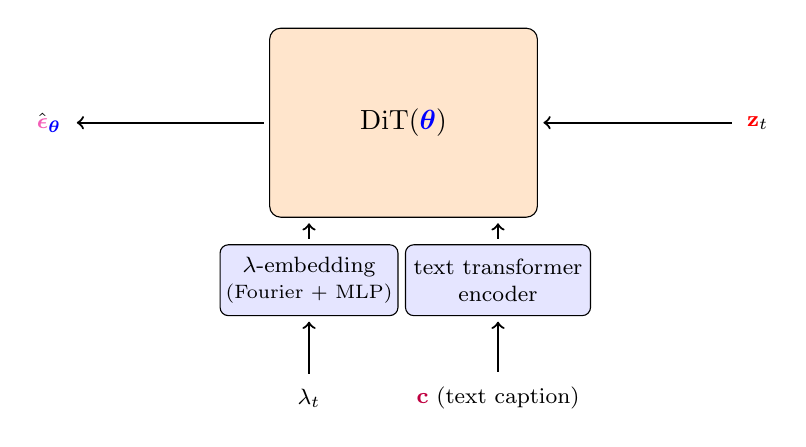
\begin{tikzpicture}[
    every node/.style={font=\small},
    dit/.style={draw, rounded corners=4pt, fill=orange!20, minimum width=3.4cm,
                minimum height=2.4cm, font=\normalsize},
    enc/.style={draw, rounded corners=3pt, fill=blue!10, minimum width=2.0cm,
                minimum height=0.9cm, inner sep=2pt, font=\footnotesize, align=center},
    sig/.style={font=\footnotesize},
    arr/.style={->, thick, shorten >=2pt, shorten <=2pt},
]
    % DiT block in the centre.
    \node[dit] (dit) at (0, 0) {$\text{DiT}(\vtheta)$};

    % z_t enters from the right.
    \node[sig] (zt) at (4.5, 0) {$\vz_t$};
    \draw[arr] (zt.west) -- (dit.east);

    % epsilon-hat exits to the left.
    \node[sig] (epshat) at (-4.5, 0) {$\hat{\vepsilon}_{\vtheta}$};
    \draw[arr] (dit.west) -- (epshat.east);

    % lambda_t enters from the bottom-left, through its encoder.
    \node[sig] (lam) at (-1.2, -3.5) {$\lambda_t$};
    \node[enc] (lamenc) at (-1.2, -2.0) {$\lambda$-embedding\\\scriptsize (Fourier + MLP)};
    \draw[arr] (lam.north) -- (lamenc.south);
    \draw[arr] (lamenc.north) -- (dit.south -| lamenc);

    % c enters from the bottom-right, through its encoder.
    \node[sig] (cc) at (1.2, -3.5) {$\vc$ (text caption)};
    \node[enc, minimum width=2.35cm] (cenc) at (1.2, -2.0) {text transformer\\encoder};
    \draw[arr] (cc.north) -- (cenc.south);
    \draw[arr] (cenc.north) -- (dit.south -| cenc);
\end{tikzpicture}
\caption{One call of the diffusion network, as used inside \texttt{ancestral\_sampling\_step}. The noisy latent $\vz_t$ enters from the right; the scalar log-SNR $\lambda_t$ and the text caption $\vc$ enter from below, after each is lifted to a feature vector / sequence by its own encoder ($\lambda$-embedding for the scalar, text transformer encoder for the caption). The DiT consumes all three and emits the predicted noise $\hat{\vepsilon}_{\vtheta}$ on the left, which is exactly the \texttt{network\_output} consumed by the sampling step. At training time, $\hat{\vepsilon}_{\vtheta}$ is compared against the true $\vepsilon_t$ via MSE; at inference time, it feeds the next sampling step. The same box, with $\hat{\vepsilon}_{\vtheta}$ swapped for $\hat{\vv}_{\vtheta}$ or $\hat{\vx}_{\vtheta}$, describes the $\vv$- and $\vx$-parameterisations introduced below.}
\label{fig:dit-training}
\end{figure}


If the models were consistent, we would expect the same relation that we used for sampling $(\vz_t = \alpha_t \vx + \sigma_t \vepsilon_t )$ to be true for the models:

\begin{align}
\vx_{\vtheta}(\vz_t,\lambda_t) = \frac{1}{\alpha_t} \left( \vz_t - \sigma_t  \vepsilon_{\vtheta}(\vz_t,\lambda_t) \right)
= \frac{1}{\alpha_t} \left( \vz_t - \sigma_t^2  \nabla_\vz \log \pT(\vz_t | \lambda_t)  \right)
\end{align}
where $\vx_{\vtheta}(\vz_t,\lambda_t)$ may be interpreted as the generated data. We can simply start from this assumption by construction.  

By predicting $\vepsilon_{\vtheta}(\vz_t,\lambda_t)$ we can reconstruct $\vx_{\vtheta}(\vz_t,\lambda_t)$. Substituting the expressions for $\vx_{\vtheta}(\vz_t,\lambda_t)$ and $\vx$ into the loss expression yields the following

\begin{align}
  \loss(\vtheta;\lambda_t)
&=
  \E
 \left\{  \frac{\alpha_t^2}{\sigma_t^4}
 \norm[\Big]{\vx_{\vtheta}(\vz_t,\lambda_t)
   - \vx }_2^2 \right\}
\nonumber
\end{align}
This loss enables us to see more clearly that we are after a model that can reconstruct the data from the noise samples $\vz$.



As pointed out by Tim Salimans and Jonathan Ho in their Progressive Distillation work for diffusion models,
when the $SNR$ is low, that is when $\sigma$ is large compared to $\alpha$, any small changes to the neural net prediction $\vepsilon_{\vtheta}(\vz_t,\lambda_t)$ will result in big changes in the reconstructions because
\begin{align}
\vx_{\vtheta}(\vz_t,\lambda_t) = \frac{1}{\alpha_t}  \vz_t - \frac{\sigma_t}{\alpha_t}  \vepsilon_{\vtheta}(\vz_t,\lambda_t).
\end{align}
The less diffusion steps (lower $T$), the bigger the problem.  To overcome this, they propose the following re-parameterisation:
\begin{align}
\vv_{\vtheta}(\vz_t,\lambda_t) = \alpha_t  \vepsilon_{\vtheta}(\vz_t,\lambda_t) - \sigma_t  \vx_{\vtheta}(\vz_t,\lambda_t)
\end{align}
 
Under this parameterisation, and with $\alpha_t^2 + \sigma_t^2 = 1$, one can easily show that:

\begin{align}
\vx_{\vtheta}(\vz_t,\lambda_t) &=  \alpha_t \vz_t - \sigma_t \vv_{\vtheta}(\vz_t,\lambda_t)
\\
\vepsilon_{\vtheta}(\vz_t,\lambda_t) &=  \sigma_t \vz_t + \alpha_t \vv_{\vtheta}(\vz_t,\lambda_t)
\end{align}
In the high-noise regime, we have
\begin{align}
\vx_{\vtheta}(\vz_t,\lambda_t) \approx -  \vv_{\vtheta}(\vz_t,\lambda_t) \hspace{.3cm} and \hspace{.3cm} \vepsilon_{\vtheta}(\vz_t,\lambda_t) \approx \vz_t.
\end{align}
On the other hand, in the low-noise regime, we have
\begin{align}
\vx_{\vtheta}(\vz_t,\lambda_t) \approx \vz_t  \hspace{.3cm} and \hspace{.3cm} \vepsilon_{\vtheta}(\vz_t,\lambda_t) \approx \vv_{\vtheta}(\vz_t,\lambda_t).
\end{align}

The first equation for $\vx_{\vtheta}(\vz_t,\lambda_t)$ will be useful for generating new data, while the one for $\vepsilon_{\vtheta}(\vz_t,\lambda_t)$ is necessary for minimizing the score matching loss.

The pytorch code for computing the loss function, using a neural network model in the same class is as follows:



\begin{minted}[fontsize=\small,
               linenos,
               breaklines,
               frame=single,
               bgcolor=black!5]{python}
Parameterisation = Literal["v", "eps"]


def diffusion_loss(
    score_network: nn.Module,
    clean_batch: Tensor,
    schedule: CosineNoiseSchedule,
    parameterisation: Parameterisation = "v",
    condition: Tensor | None = None,
) -> Tensor:
    """Denoising score-matching loss for a diffusion model.

    For each sample in the batch we draw an independent time t ~ U[0, 1],
    add the corresponding noise, ask the network for either the noise or
    the velocity, convert to a noise prediction, and compute MSE against
    the true noise.
    """
    batch_size = clean_batch.shape[0]
    device = clean_batch.device

    # Sample one t per example, then look up alpha_t, sigma_t, lambda_t.
    t = torch.rand(batch_size, device=device)
    log_snr_t = schedule.log_snr(t)
    alpha_t, sigma_t = schedule.alpha_sigma(log_snr_t)

    # Reshape the schedule scalars so they broadcast over the feature dims.
    feature_shape = (-1,) + (1,) * (clean_batch.ndim - 1)
    alpha_t = alpha_t.view(feature_shape)
    sigma_t = sigma_t.view(feature_shape)

    # Forward noising.
    noisy_sample, true_noise = add_noise(clean_batch, alpha_t, sigma_t)

    # Network forward pass.
    network_output = score_network(noisy_sample, log_snr_t, condition)

    # Convert whatever the network predicts into a noise prediction so we can
    # compare against `true_noise` with the same loss in both parameterisations.
    if parameterisation == "v":
        predicted_noise = sigma_t * noisy_sample + alpha_t * network_output
    elif parameterisation == "eps":
        predicted_noise = network_output
    else:
        raise ValueError(f"Unknown parameterisation: {parameterisation!r}")

    return F.mse_loss(predicted_noise, true_noise)
\end{minted}
The code above allows one to use the epsilon-parameterisation or the v-parameterisation.
This is all we need to train the model, which can be a UViT, a UNet or any transformer. We simply need to minimize this loss to learn the neural net parameters.

The model can also have \emph{control inputs}, which can be a text prompt, quality score, camera motion, previous or future frames of a video, and so on.

Next, we discuss inference, that is how to start at noise and then progressively sample new images in the reverse process.












\section{Inference}


Our way of sampling, can been seen as a forward noising mechanism:
\begin{align}
\vz_t \sim q(\vz_t|\vx) = \gauss(\vz_t|\alpha_t \vx, \sigma_t^2 \vI)
\nonumber
\end{align}
Using Bayes' rule, we can obtain a way of sampling backward, to eliminate the noise as follows:

\begin{align}
q(\vz_{t}|\vz_{t+1},\vx) = \frac{q(\vz_{t+1}|\vz_{t},\vx)q(\vz_{t}|\vx)}{q(\vz_{t+1}|\vx)}
= \frac{q(\vz_{t+1}|\vz_{t})q(\vz_{t}|\vx)}{q(\vz_{t+1}|\vx)}
\nonumber
\end{align}
With a Markovian forward process, we have $q(\vz_{t+1}|\vz_{t},\vx)=q(\vz_{t+1}|\vz_{t})$. The distributions $q(\vz_{t}|\vx)$ and $q(\vz_{t+1}|\vx)$ are Gaussian by definition. It can be shown that the distribution $q(\vz_{t+1}|\vz_{t})$ is also Gaussian.  Specifically,

\begin{align}
q(\vz_{t+1}|\vz_{t}) = \mathcal{N}\left(\vz_{t+1};  \frac{\alpha_{t+1}}{\alpha_t} \vz_{t},   \sigma_{t+1}^2 - \frac{\alpha_{t+1}^2}{\alpha_t^2} \sigma_t^2  \vI\right)
\end{align}
To see this, note that unrolling this expression we have:

\begin{align}
\vz_{t+1} &= \frac{\alpha_{t+1}}{\alpha_t} \vz_{t} + \sqrt{\sigma_{t+1}^2 - \frac{\alpha_{t+1}^2}{\alpha_t^2} \sigma_t^2} \vepsilon_{t+1} \nonumber \\
&= \frac{\alpha_{t+1}}{\alpha_t} \frac{\alpha_{t}}{\alpha_{t-1}} \vz_{t-1} +  \frac{\alpha_{t+1}}{\alpha_t}  \sqrt{\sigma_{t}^2 - \frac{\alpha_{t}^2}{\alpha_{t-1}^2} \sigma_{t-1}^2} \vepsilon_{t} + \sqrt{\sigma_{t+1}^2 - \frac{\alpha_{t+1}^2}{\alpha_t^2} \sigma_t^2} \vepsilon_{t+1} \nonumber \\
&= \frac{\alpha_{t+1}}{\alpha_{t-1}} \vz_{t-1} +    \sqrt{\sigma_{t+1}^2 - \frac{\alpha_{t+1}^2}{\alpha_{t-1}^2} \sigma_{t-1}^2} \tilde{\vepsilon}_{t+1} \nonumber
\end{align}
where to get the last line we have used that the sum of two normal random variables is normal with the appropriate parameters. Intuitively, if we continue expanding this recursion we will arrive at our expression for $q(\vz_t|\vx) = \gauss(\vz_t|\alpha_t \vx, \sigma_t^2 \vI)$ as expected:

\begin{align}
\vz_{t+1} &=  \frac{\alpha_{t+1}}{\alpha_{0}} \vz_{0} +   \sqrt{\sigma_{t+1}^2 - \frac{\alpha_{t+1}^2}{\alpha_{0}^2} \sigma_{0}^2} \tilde{\vepsilon}_{t+1} \nonumber \\
&=  \alpha_{t+1} \vz_{0} + \sigma_{t+1} \tilde{\vepsilon}_{t+1} \nonumber \\
&=  \alpha_{t+1} \vx + \sigma_{t+1} \tilde{\vepsilon}_{t+1} \nonumber
\end{align}
We have used the fact that by construction, when the noise vanishes, we have $\alpha_0 = 1$, $\sigma_0 = 0$ and $\vz_0 = \vx$.

We can now apply Bayes' rule to obtain an expression for the normal distribution $q(\vz_{t}|\vz_{t+1},\vx)$. The algebra involved in this is about completing the square of the exponent of the Gaussian. There is a derivation of this in the Appendix.

The resulting Gaussian distribution is:

\begin{align}
q(\vz_{t}|\vz_{t+1}, \vx) &= \mathcal{N}\left(\vz_{t};  
\frac{\alpha_{t+1}}{\alpha_{t}} \frac{\sigma_{t}^2}{\sigma_{t+1}^2} \vz_{t+1}
+ \left(\sigma_{t+1}^2 - \frac{\alpha_{t+1}^2}{\alpha_t^2} \sigma_t^2\right)  \frac{\alpha_{t}}{\sigma^2_{t+1}} \vx,
\left(\sigma_{t+1}^2 - \frac{\alpha_{t+1}^2}{\alpha_t^2} \sigma_t^2\right) \frac{\sigma_{t}^2}{\sigma_{t+1}^2} \vI\right) \nonumber \\
&=
\mathcal{N}\left(\vz_{t};  
\frac{\alpha_{t}}{\alpha_{t+1}} \frac{\alpha_{t+1}^2}{\sigma_{t+1}^2} \frac{\sigma_{t}^2}{\alpha_{t}^2} \vz_{t+1}
+ \left(1 - \frac{\alpha_{t+1}^2}{\sigma_{t+1}^2} \frac{\sigma_t^2}{\alpha_t^2}\right)  \alpha_{t} \vx,
\left( 1 - \frac{\alpha_{t+1}^2}{\sigma_{t+1}^2} \frac{\sigma_t^2}{\alpha_t^2}\right) \sigma_{t}^2
\vI\right) \nonumber \\
&=
\mathcal{N}\left(\vz_{t};  
\frac{\alpha_{t}}{\alpha_{t+1}}
e^{\lambda_{t+1} - \lambda_t }
\vz_{t+1}
+ \left(1 - e^{\lambda_{t+1} - \lambda_t } \right)  \alpha_{t} \vx,
\left(1 - e^{\lambda_{t+1} - \lambda_t } \right) \sigma_{t}^2
\vI\right) \nonumber \\
&=
\mathcal{N}\left(\vz_{t};  
\alpha_{t} \left[
\frac{(1-c)}{\alpha_{t+1}}
\vz_{t+1}
+ c \vx \right],
c \sigma_{t}^2
\vI\right)
\end{align}
where we used the notation $\lambda_t = \log \alpha_t^2/\sigma_t^2$ for the log SNR.
The above distribution is what we use for drawing samples. We use the score matching loss to learn the approximation

\begin{align}
\vx_{\vtheta}(\vz_t,\lambda_t) &=  \alpha_t \vz_t - \sigma_t \vv_{\vtheta}(\vz_t,\lambda_t)
\end{align}
and replace $\vx_{t}$ with $\vx_{\vtheta}(\vz_t,\lambda_t)$ in $q(\vz_{t}|\vz_{t+1}, \vx)$ in order to draw novel samples. That is,
\begin{align}
q(\vz_{t}|\vz_{t+1}, \vx) &=
\mathcal{N}\left(\vz_{t};  
\alpha_{t} \left[
\frac{(1-c)}{\alpha_{t+1}}
\vz_{t+1}
+ c \vx_{\vtheta}(\vz_{t+1},\lambda_{t+1})\right],
c \sigma_{t}^2
\vI\right)
\end{align}





In code, we implement this with the following two functions:



\begin{minted}[fontsize=\small,
               linenos,
               breaklines,
               frame=single,
               bgcolor=black!5]{python}
@torch.no_grad()
def ancestral_sampling_step(
    noisy_sample: Tensor,
    network_output: Tensor,
    log_snr_t: Tensor,
    log_snr_s: Tensor,
    parameterisation: Parameterisation,
    clip_to: tuple[float, float] | None = (-1.0, 1.0),
) -> tuple[Tensor, Tensor]:
    """One reverse step of ancestral sampling, from noise level t down to s < t.

    Returns the mean and (scalar) variance of q(z_s | z_t, x_hat), where
    x_hat is reconstructed from the network output.
    """
    # -expm1(x) = 1 - exp(x); positive when log_snr_t < log_snr_s.
    c = -torch.expm1(log_snr_t - log_snr_s)

    alpha_t = torch.sqrt(torch.sigmoid(log_snr_t))
    alpha_s = torch.sqrt(torch.sigmoid(log_snr_s))
    sigma_t = torch.sqrt(torch.sigmoid(-log_snr_t))
    sigma_s = torch.sqrt(torch.sigmoid(-log_snr_s))

    # Decode the network output into a prediction of the clean sample x.
    if parameterisation == "v":
        predicted_clean = alpha_t * noisy_sample - sigma_t * network_output
    elif parameterisation == "eps":
        predicted_clean = (noisy_sample - sigma_t * network_output) / alpha_t
    else:
        raise ValueError(f"Unknown parameterisation: {parameterisation!r}")

    if clip_to is not None:
        predicted_clean = predicted_clean.clamp(*clip_to)

    posterior_mean = alpha_s * (
        noisy_sample * (1.0 - c) / alpha_t + c * predicted_clean
    )
    posterior_variance = (sigma_s ** 2) * c
    return posterior_mean, posterior_variance
\end{minted}

The corresponding code is just a Python \texttt{for} loop over timesteps, calling the same network at each iteration:

\begin{minted}[fontsize=\small,
               linenos,
               breaklines,
               frame=single,
               bgcolor=black!5]{python}
@torch.no_grad()
def generate_samples(
    score_network: nn.Module,
    schedule: CosineNoiseSchedule,
    sample_shape: tuple[int, ...],
    num_steps: int = 100,
    parameterisation: Parameterisation = "v",
    condition: Tensor | None = None,
    clip_to: tuple[float, float] | None = None,
    device: torch.device = DEVICE,
) -> Tensor:
    """Generate a batch of samples by running ancestral sampling end-to-end.

    Starts from pure Gaussian noise at t=1 and iterates the reverse step
    down to t=0 on a uniform grid of `num_steps` points.
    """
    sample = torch.randn(sample_shape, device=device)

    for step in reversed(range(1, num_steps + 1)):
        t_now = torch.tensor(step / num_steps, device=device)
        t_next = torch.tensor((step - 1) / num_steps, device=device)

        log_snr_t = schedule.log_snr(t_now)
        log_snr_s = schedule.log_snr(t_next)

        # The network expects a per-sample log-SNR; broadcast the scalar.
        log_snr_t_batched = log_snr_t.expand(sample.shape[0])
        network_output = score_network(sample, log_snr_t_batched, condition)

        mean, variance = ancestral_sampling_step(
            noisy_sample=sample,
            network_output=network_output,
            log_snr_t=log_snr_t,
            log_snr_s=log_snr_s,
            parameterisation=parameterisation,
            clip_to=clip_to,
        )

        if step > 1:
            # Stochastic step: add noise scaled by sqrt(variance).
            sample = mean + torch.randn_like(mean) * torch.sqrt(variance)
        else:
            # Last step: take the mean (deterministic) to avoid noisy outputs.
            sample = mean

    return sample
\end{minted}

During generation, it is helpful to clip the predicted clean sample $\hat{\vx}$ in $\vx$-space, which the \texttt{ancestral\_sampling\_step} function above does via the \texttt{clip\_to} argument (e.g.\ \texttt{clip\_to=(-1, 1)} when the data is normalised to $[-1, 1]$).

The structure of the loop in \texttt{generate\_samples} above is exactly that of an unrolled recurrent network with tied parameters: the same DiT (same $\vtheta$) is called at every step, the only things that change between steps are the latent $\vz_t$ and the noise level $\lambda_t$. Figure~\ref{fig:dit-unrolled} unrolls four iterations of the loop.




\begin{figure}[H]
\centering
\resizebox{\textwidth}{!}{%
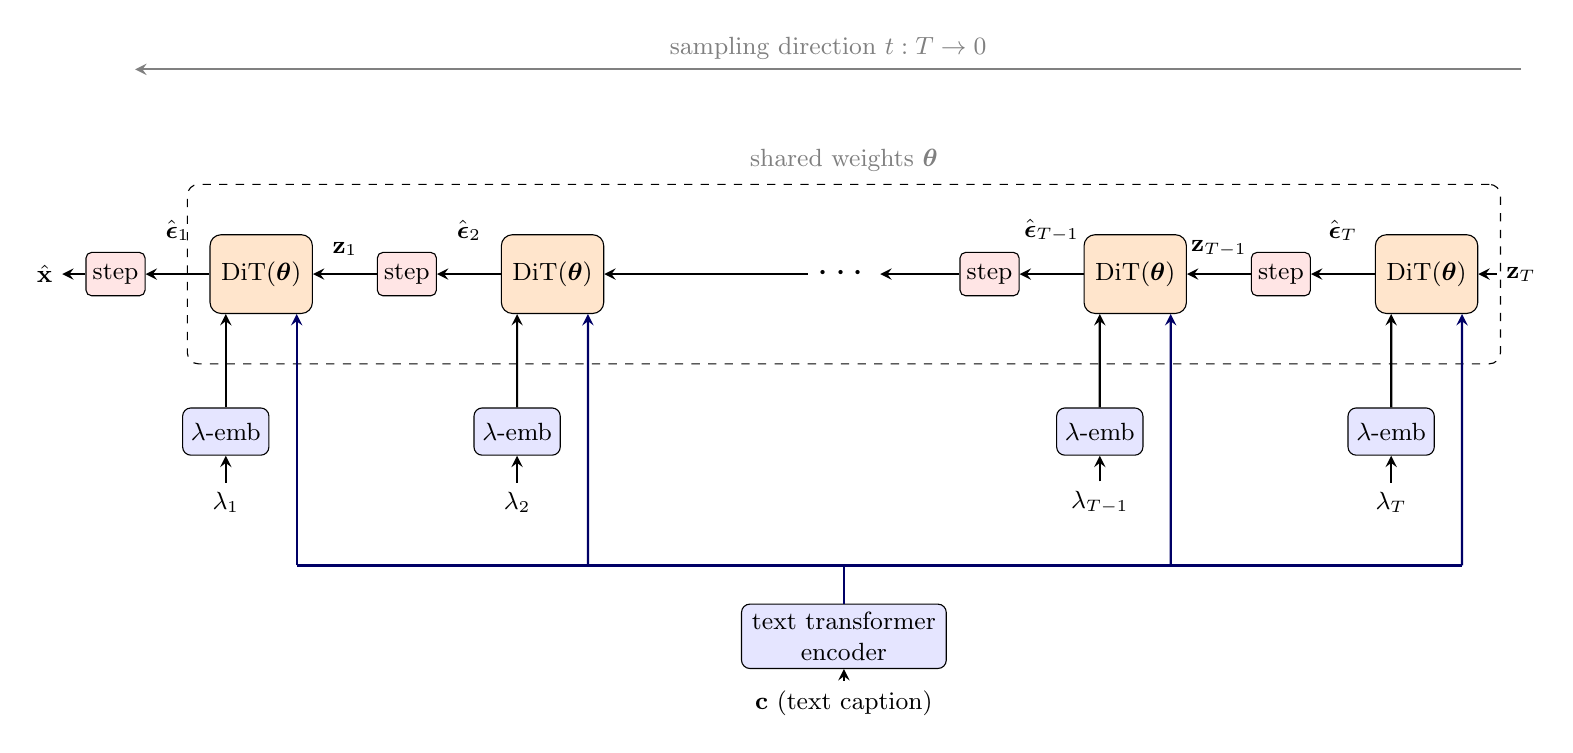
\begin{tikzpicture}[
    every node/.style={font=\normalsize},
    dit/.style={draw, rounded corners=4pt, fill=orange!20, minimum width=1.3cm,
                minimum height=1.0cm, font=\small, inner sep=2pt},
    enc/.style={draw, rounded corners=3pt, fill=blue!10, inner sep=3pt,
                font=\small, align=center, minimum width=1.0cm, minimum height=0.6cm},
    stepbox/.style={draw, rounded corners=2pt, fill=red!10, minimum width=0.75cm,
                 minimum height=0.55cm, font=\small, inner sep=2pt},
    sig/.style={font=\small},
    arr/.style={->, >=stealth, thick},
    arrg/.style={->, >=stealth, gray, thick},
    cbus/.style={->, >=stealth, blue!40!black, thick},
]
    % --- Geometry ---
    % We use explicit x-coordinates for each column so the middle gap stays tight.
    % Right cluster: step T and step T-1 (DiTs d5, d4 with step boxes s5, s4)
    % Left  cluster: step 2 and step 1 (DiTs d2, d1 with step boxes s2, s1)
    % Between them: a single \cdots node.
    \def\dx{3.7}                 % spacing between adjacent DiT centres within a cluster
    \def\dity{0}
    \def\zy{0}
    \def\encyl{-2.0}             % lambda-encoder y
    \def\sigyl{-2.9}             % lambda symbol y
    \def\busy{-3.7}              % c-bus y
    \def\encyc{-4.6}             % text-encoder y
    \def\loff{-0.45}             % lambda-emb x-offset from DiT centre
    \def\coff{0.45}              % c-bus entry x-offset from DiT centre
    \def\stepx{1.85}             % step box x-distance to LEFT of each DiT centre
    \def\epsy{0.55}              % y-position for eps-hat labels

    % Cluster x-coordinates (left cluster centred on x=1*\dx and 2*\dx,
    % right cluster centred on x=4*\dx and 5*\dx; middle dots at midpoint)
    \def\xL{0}        % d1 x
    \def\xLb{\dx}     % d2 x
    \def\xMid{2*\dx}  % middle dots x
    \def\xRb{3*\dx}   % d4 x
    \def\xR{4*\dx}    % d5 x (above wire, below envelope top)

    % --- DiT blocks ---
    \node[dit] (d5) at (\xR,  \dity) {$\text{DiT}(\boldsymbol{\theta})$};
    \node[dit] (d4) at (\xRb, \dity) {$\text{DiT}(\boldsymbol{\theta})$};
    \node[dit] (d2) at (\xLb, \dity) {$\text{DiT}(\boldsymbol{\theta})$};
    \node[dit] (d1) at (\xL,  \dity) {$\text{DiT}(\boldsymbol{\theta})$};

    % --- Endpoints on the wire ---
    \node[sig] (zT)   at (\xR + 1.2, \zy) {$\mathbf{z}_T$};
    \node[sig] (xhat) at (\xL - \stepx - 0.9, \zy) {$\hat{\mathbf{x}}$};

    % --- step boxes ---
    \node[stepbox] (s5) at (\xR  - \stepx, \dity) {step};
    \node[stepbox] (s4) at (\xRb - \stepx, \dity) {step};
    \node[stepbox] (s2) at (\xLb - \stepx, \dity) {step};
    \node[stepbox] (s1) at (\xL  - \stepx, \dity) {step};

    % --- Middle dots for omitted steps ---
    \node[sig, font=\Large] (middledots) at (\xMid, \dity) {$\cdots$};

    % ===== Arrows =====
    % Each step has: z_t -> DiT, then DiT -> step box (with eps-hat label above),
    % then step -> next z_{t-1}. Arrows STOP at the step box (arrowhead INTO the box),
    % and a new arrow leaves OUT of the box. eps-hat labels sit above the wire so
    % they cannot collide with the step box on the row.

    % --- Step T ---
    \draw[arr] (zT.west) -- (d5.east);
    \draw[arr] (d5.west) -- (s5.east);
    \node[font=\small] at ($(d5.west)!0.5!(s5.east) + (0,\epsy)$) {$\hat{\boldsymbol{\epsilon}}_T$};
    \draw[arr] (s5.west) -- (d4.east);
    \node[sig] at ($(s5.west)!0.5!(d4.east) + (0,0.32)$) {$\mathbf{z}_{T-1}$};

    % --- Step T-1 ---
    \draw[arr] (d4.west) -- (s4.east);
    \node[font=\small] at ($(d4.west)!0.5!(s4.east) + (0,\epsy)$) {$\hat{\boldsymbol{\epsilon}}_{T-1}$};
    \draw[arr] (s4.west) -- (middledots.east);
    \draw[arr] (middledots.west) -- (d2.east);

    % --- Step 2 ---
    \draw[arr] (d2.west) -- (s2.east);
    \node[font=\small] at ($(d2.west)!0.5!(s2.east) + (0,\epsy)$) {$\hat{\boldsymbol{\epsilon}}_{2}$};
    \draw[arr] (s2.west) -- (d1.east);
    \node[sig] at ($(s2.west)!0.5!(d1.east) + (0,0.32)$) {$\mathbf{z}_{1}$};

    % --- Step 1 ---
    \draw[arr] (d1.west) -- (s1.east);
    \node[font=\small] at ($(d1.west)!0.5!(s1.east) + (0,\epsy)$) {$\hat{\boldsymbol{\epsilon}}_{1}$};
    \draw[arr] (s1.west) -- (xhat.east);

    % --- Per-step lambda encoders ---
    \node[enc] (le5) at (\xR  + \loff, \encyl) {$\lambda$-emb};
    \node[enc] (le4) at (\xRb + \loff, \encyl) {$\lambda$-emb};
    \node[enc] (le2) at (\xLb + \loff, \encyl) {$\lambda$-emb};
    \node[enc] (le1) at (\xL  + \loff, \encyl) {$\lambda$-emb};

    \node[sig] (lT) at (\xR  + \loff, \sigyl) {$\lambda_T$};
    \node[sig] (l4) at (\xRb + \loff, \sigyl) {$\lambda_{T-1}$};
    \node[sig] (l2) at (\xLb + \loff, \sigyl) {$\lambda_{2}$};
    \node[sig] (l1) at (\xL  + \loff, \sigyl) {$\lambda_{1}$};

    \draw[arr] (lT.north) -- (le5.south); \draw[arr] (le5.north) -- ($(d5.south) + (\loff,0)$);
    \draw[arr] (l4.north) -- (le4.south); \draw[arr] (le4.north) -- ($(d4.south) + (\loff,0)$);
    \draw[arr] (l2.north) -- (le2.south); \draw[arr] (le2.north) -- ($(d2.south) + (\loff,0)$);
    \draw[arr] (l1.north) -- (le1.south); \draw[arr] (le1.north) -- ($(d1.south) + (\loff,0)$);

    % --- Text transformer encoder + horizontal bus ---
    \node[enc, minimum width=2.6cm] (cenc) at (\xMid, \encyc) {text transformer\\encoder};
    \node[sig, anchor=north] (cc) at ($(cenc.south) + (0,-0.15)$) {$\mathbf{c}$ (text caption)};
    \draw[arr] (cc.north) -- (cenc.south);

    \draw[blue!40!black, thick] (cenc.north) -- (\xMid, \busy);
    \draw[blue!40!black, thick] (\xL + \coff, \busy) -- (\xR + \coff, \busy);
    \draw[cbus] (\xL  + \coff, \busy) -- ($(d1.south) + (\coff,0)$);
    \draw[cbus] (\xLb + \coff, \busy) -- ($(d2.south) + (\coff,0)$);
    \draw[cbus] (\xRb + \coff, \busy) -- ($(d4.south) + (\coff,0)$);
    \draw[cbus] (\xR  + \coff, \busy) -- ($(d5.south) + (\coff,0)$);

    % --- Shared-weights envelope ---
    \begin{scope}[on background layer]
        \node[draw, dashed, rounded corners=4pt,
              fit=(d1)(d2)(d4)(d5)(middledots), inner ysep=18pt, inner xsep=8pt] (env) {};
    \end{scope}
    \node[font=\small, gray] at ($(env.north) + (0,0.3)$) {shared weights $\boldsymbol{\theta}$};

    % --- Time-axis arrow above ---
    \draw[->, >=stealth, gray, thick] (\xR + 1.2, 2.6) --
          node[above, font=\small, gray]{sampling direction $t: T \to 0$}
          (\xL - 1.6, 2.6);
\end{tikzpicture}%
}
\caption{Inference (\texttt{generate\_samples}) unrolled as a tied-parameter recurrent neural network (RNN). The \emph{same} DiT (same weights $\boldsymbol{\theta}$) is applied at every step; what changes between steps is (i) the input latent $\mathbf{z}_t$ on the right of each block and (ii) the noise level $\lambda_t$ injected from below through the $\lambda$-embedding (one fresh $\lambda_t$ per step). The text caption $\mathbf{c}$ is encoded \emph{once} by a text transformer encoder and the same conditioning is fanned out (blue bus) to every DiT call. Each DiT emits a noise prediction $\hat{\boldsymbol{\epsilon}}_t$, which is consumed by the small red \texttt{step} box. This is exactly \texttt{ancestral\_sampling\_step}. Time runs right-to-left: we start from pure Gaussian noise $\mathbf{z}_T$ on the right and, after $T$ DiT calls, read off the generated sample $\hat{\mathbf{x}} = \mathbf{z}_0$ on the left.}
\label{fig:dit-unrolled}
\end{figure}








\paragraph{Connection to looped and feedback language models.}
Figure~\ref{fig:dit-unrolled} is also a useful way to view recent recurrent-depth LLMs.  The diffusion sampler is a \emph{loop over latent state}: the same transformer weights are reused, and each pass refines a hidden object, here the noisy latent $\vz_t$.  In \href{https://arxiv.org/abs/2510.25741}{Looped Language Models} (Zhu et al., 2025), the same idea is applied inside an LLM: a shared recurrent block performs several latent ``thinking'' updates before emitting tokens, and the model can allocate more recurrent depth to harder examples.  Earlier, the \href{https://arxiv.org/abs/2002.09402}{Feedback Transformer} (Fan et al., 2020) used a related feedback idea along the sequence direction: future token representations can read high-level representations computed for previous tokens, rather than only lower-layer states.  The analogy is not exact, but it is instructive.  In Figure~\ref{fig:dit-unrolled}, the recurrence index is diffusion time and the state is an external sample $\vz_t$; in looped LLMs the recurrence index is latent reasoning depth; in feedback transformers the recurrent signal is memory from earlier sequence positions.  In all three cases, the core move is parameter sharing across repeated computation, which turns a feed-forward transformer block into an iterative refinement machine.


\section{The important details}

The preceding two sections have all the code needed to train a diffusion model, and to generate new images with it at inference time.
Some details are missing. Sometimes we use encoders and decoders to project the images and videos to lower dimensional spaces. We have abstracted all the details of the neural network model, and in particular how we condition. We have not discussed the effect of scale. Most importantly, we have not discussed data. Getting good captions for the images and conditioning on these is of paramount importance to attain SoTA models.






























\subsection{Classifier free guidance}
Typically we have text captions $c$ and want to generate images or videos that match such captions. In \emph{classifier-free guidance}, we use Bayes' rule to compute
$p(\vy|\vx) =  p(\vx|\vy) p(\vy)/ p(\vx)$,
and hence
\be
\log p(\vy|\vx) = \log p(\vx|\vy)  + \log p(\vy) - \log p(\vx)
\ee
so the score of the induced classifier becomes
\be
\nabla_{\vx} \log p(\vy|\vx) = \nabla_{\vx} \log p(\vx|\vy)  - \nabla_{\vx} \log p(\vx)
\ee
Plugging in the scaled guidance signal gives
\begin{align}
\nabla_{\vx} \log p_{w}(\vx|\vy)
&= \nabla_{\vx} \log p(\vx)  + w(\nabla_{\vx} \log p(\vx|\vy)  - \nabla_{\vx} \log p(\vx)) \\
&= (1-w) \nabla_{\vx} \log p(\vx)  + w \nabla_{\vx} \log p(\vx|\vy)
\end{align}
For $w=0$ we recover the unconditional model, and for $w=1$ we recover
the standard conditional model.

In practice, we can implement this method with a small change
to the ancestral sampling routine.
At each step $t$, we predict the guided error term,
which has the form
\be
% Before Yannis' fix: \tilde{\vepsilon}_t  = \weight \vepsilon_{\vtheta}(\vz_t,t,c)
\tilde{\vv}_t  = w \vv_{\vtheta}(\vz_t,\lambda_t,\vy)
+ (1-w) \vv_{\vtheta}(\vz_t,\lambda_t,\emptyset)
\ee
That is, instead of training a conditional and unconditional model,
 we can just train a single conditional model,
provided we  set $\vy=\emptyset$ with probability $1-w$ to emulate unconditional sampling.
The advantage of this approach is that we have a single, self-consistent model,
where the guidance signal is derived from a generative model,
for which gradients in input space are more meaningful.


\subsection{Classifier guidance}

An alternative to introduce guidance, is to replace $\vx_{\vtheta}(\vz_t,\lambda_t, \vy_t)$ with the corresponding score parameterisation:
\begin{align}
q(\vz_{t}|\vz_{t+1}, \vx) &=
\mathcal{N}\left(\vz_{t};  
\alpha_{t} \left[
\frac{(1-c)}{\alpha_{t+1}}
\vz_{t+1}
+ c \vx_{\vtheta}(\vz_{t+1},\lambda_{t+1},\vy)\right],
c \sigma_{t}^2
\vI\right) \nonumber \\
&=
\mathcal{N}\left(\vz_{t};  
\left[
\frac{\alpha_{t} (1-c)}{\alpha_{t+1}}
\vz_{t+1}
+ c  \left( \vz_{t+1} - \sigma_t^2  \nabla_\vz \log \pT(\vz_{t+1}|\lambda_{t+1},\vy)  \right)\right],
c \sigma_{t}^2
\vI\right) \nonumber \\
& \equiv
\mathcal{N}\left(\vz_{t};  
\left[
\frac{\alpha_{t} (1-c)}{\alpha_{t+1}}
\vz_{t+1}
+ c  \left( \vz_{t+1} - \sigma_t^2 ( \nabla_\vz \log \pT(\vz_{t+1}|\lambda_{t+1}) + \nabla_\vz \log \pT(\vy | \vz_{t+1} ) ) \right)\right],
c \sigma_{t}^2
\vI\right) \nonumber
\end{align}

The challenge with this approach is that we need to train a classifier $\pT(\vy | \vz_{t+1} )$ that works well for each level of noise. This is a lot like the old inception work of Google -- look for those inception patterns in generated images to reveal whether this technique has been used.


\section{Connection with DDPM parameterisation}

We started with the forward equation
\begin{align}
\vz_t = \alpha_t \vx + \sigma_t \vepsilon_t \nonumber
\end{align}
and derived the following two expressions:
\be
q(\vz_{t+1} | \vz_t) = \gauss\left(\frac{\alpha_{t+1}}{\alpha_t} \vz_t, \left(\sigma_{t+1}^2 - \frac{\alpha_{t+1}^2}{\alpha_t^2}\sigma_t^2\right) \vI\right) \nonumber
\ee
and
\begin{align}
q(\vz_{t}|\vz_{t+1}, \vx) &= \mathcal{N}\left(
\frac{\alpha_{t+1}}{\alpha_{t}} \frac{\sigma_{t}^2}{\sigma_{t+1}^2} \vz_{t+1}
+ \left(\sigma_{t+1}^2 - \frac{\alpha_{t+1}^2}{\alpha_t^2} \sigma_t^2\right)  \frac{\alpha_{t}}{\sigma^2_{t+1}} \vx,
\left(\sigma_{t+1}^2 - \frac{\alpha_{t+1}^2}{\alpha_t^2} \sigma_t^2\right) \frac{\sigma_{t}^2}{\sigma_{t+1}^2} \vI\right) \nonumber
\end{align}




A lot of \href{https://arxiv.org/abs/2006.11239}{denoising diffusion probabilistic model (DDPM)} papers, including Dall-e start with the forward process:  
\begin{align}
\vz_t = \sqrt{\rho_t} \vx + \sqrt{1 - \rho_t}  \vepsilon_t \nonumber
\end{align}
and derive
\be
q(\vz_{t+1} | \vz_t) = \gauss\left( \sqrt{1-\beta_{t+1}} \vz_t, \beta_{t+1}  \vI\right) \nonumber
\ee
and
\begin{align}
q(\vz_{t-1}|\vz_{t}, \vx) &= \mathcal{N}\left(
\frac{1-\rho_{t-1}}{1-\rho_t} \sqrt{1-\beta_t} \vz_{t}
+   \frac{\sqrt{\rho_{t-1}} \beta_t}{ 1-\rho_t} \vx,
 \frac{\beta_t(1-\rho_{t-1})}{1-\rho_t} \vI\right) \nonumber
\end{align}

However, these two derivations are the same, when one uses the following correspondences:
\be
\sqrt{\rho_t} = \alpha_t, \sigma_t = \sqrt{1-\rho_t}, \sqrt{1-\beta_t} = \frac{\alpha_t}{\alpha_{t-1}}, \beta_t = \sigma_t^2 - \frac{\alpha_t^2}{\alpha_{t-1}^2} \sigma_{t-1}^2
\ee




\section{The conditional expectation trick}


One of the most widely used tricks in the theory of diffusion and flow matching is the definition of conditional expectation. Specifically, if
\be
\vy = f(\vu)  = \E [\vx | \vu ]
\ee
Then the optimal solution $f$ is the one that minimizes
\be
\hat{f} = \arg \min_f \E [\norm{\vx - f( \vu )}^2]
\ee
and vice versa.

For example, at the start, we derived the following loss:
\begin{align}
  \loss(\vtheta;\lambda_t)
&=
 \E
 \left\{  
 \norm[\Big]{\vs_{\vtheta}(\vz_t,\lambda_t)
   + \frac{1}{\sigma_t}\vepsilon_t }_2^2 \right\}
\nonumber
\end{align}
From our conditional expectation result, we obtain:
\be
\vs_{\vtheta}(\vz_t,\lambda_t) = - \frac{1}{\sigma_t} \E[ \vepsilon_t | \vz_t ]
\ee

This trick will turn out to be super helpful to derive probability flow matching in the next section.


\section{Flow matching}

\subsection{The key insight}
Flow matching is based on the following important theoretical result, which we prove in Appendix B. The marginal probability distribution $p_t(\vz)$ associated with the samples generated according to our forward diffusion process
\begin{align}
\vz_t = \alpha_t \vx + \sigma_t \vepsilon_t \nonumber
\end{align}
is the same as the distribution of the probability flow ODE with velocity field:
\begin{align}
 \frac{d\vz(t)}{dt} = \dot{\vz}_t =  \vv(\vz, t)
\end{align}
where the vector field $\vv(\vz, t) $ (\emph{not to be confused by the v-parameterisation in diffusion - sorry!}) is given by the conditional expectation
\begin{align}
\vv(\vz, t) &= \mathbb{E}[\dot{\vz}_t | \vz_t = \vz] \nonumber \\
&= \dot{\alpha}_t \mathbb{E}[\vx | \vz_t = \vz] + \dot{\sigma}_t \mathbb{E}[\vepsilon | \vz_t = \vz].
\end{align}
This velocity field governs the deterministic transport of the probability density, ensuring that the evolution of the unique \( p_t(\vz) \) backward from $t=T$, (which is governed by an ODE with known initial conditions at $t=T$) matches that of the forward diffusion process. By solving the probability flow ODE backward in time from \( \vz_T = \vepsilon \sim \mathcal{N}(\vzero, \vI) \), we can generate samples from \( p_0(\vx) \), which approximates the true data distribution \( p(\vx) \).

In short, the distribution over the images generated by the forward diffuse process is the same as the distribution over the images generated by following the ODE.
We simply need to run an ODE numerical technique with a parameterised field $ \vv_{\vtheta}(\vz, t) $ in order to draw samples. This is how we will do the inference step. That is, instead of deriving Gaussian distributions as done for diffusion, we will simply use an available ODE solver.

The ODE can be discretised with the Euler method, resulting in a simple algorithm over a discrete grid:
\be
\vz_{i+1} = \vz_{i} + \eta \vv_{\vtheta}(\vz_i, t_i)
\ee
In practice, we simply use one of the many existing ODE solver packages.

\subsection{Flow matching training}

For training, we use the conditional expectation trick from the previous section. Since $\vv(\vz, t) = \dot{\alpha}_t \mathbb{E}[\vx | \vz_t = \vz] + \dot{\sigma}_t \mathbb{E}[\vepsilon | \vz_t = \vz]$, we can obtain the neural network $ \vv_{\vtheta}(\vz, t) $ by minimizing:
\begin{align}
  \loss_{v}(\vtheta;t)
&=
 \E
 \left\{  
 \norm[\Big]{\vv_{\vtheta}(\vz_t,t)
   - \dot{\alpha}_t \vx - \dot{\sigma}_t \vepsilon_t
   }_2^2
   \right\}
\nonumber
\end{align}
Choosing a linear schedule $\alpha_t = 1-t$ and $\beta_t = t$ between 0 and 1, we have $\dot{\alpha}_t = -1$ and $\dot{\sigma}_t = 1$, so $\dot{\alpha}_t \vx + \dot{\sigma}_t \vepsilon_t = \vepsilon_t - \vx$. The loss then becomes the usual expression also found in the rectified flow papers:
\begin{align}
  \loss_{v}(\vtheta)
&=
 \E
 \left\{  
 \norm[\Big]{\vv_{\vtheta}(\vz_t,t,\vc)
   -  (\vepsilon_t - \vx)
   }_2^2
   \right\}
\nonumber
\end{align}
We could have also used $\alpha_t = \cos(1/2\pi t)$ and $\beta_t = \sin (1/2 \pi t)$, but the linear parameterisation results in a very simple objective function.

For the code, I will use the \href{https://arxiv.org/abs/2210.02747}{conditional flow matching (CFM)} variant which Meta uses. It is the same as what I derived but, annoyingly, the image is defined as \[\vx = \vz_1\] and noise \[\vepsilon = \vz_0\] with $\alpha_t = t$ and $\beta_t = 1-t$. That is, the direction is inverted. I could have undone this, but it's rather painful so from now on in this section and the flow matching inference section only we reverse the direction of denoising (to backward) and generation (to forward).    

CFM uses the intermediate definition:
\be
\vvarphi_t (\vz_0, \vz_1) = (1 - (1 - \sigma_{min})t)\vz_0 + t \vz_1
\ee
with $\vepsilon = \vz_{0}$. Here, $\sigma_{min}$ is a tiny number. Then the loss becomes
\begin{align}
  \loss_{v}(\vtheta)
&= \E_{t}
 \E_{\vx \sim p_d(\vx)}
 \E_{\vz_0 \sim \gauss(\vzero,\vI)}
 \left\{  
 \norm[\Big]{\vv_{\vtheta}(\vvarphi_t (\vz_0, \vz_1))
   -  (\vz_1 - (1 - \sigma_{min})\vz_0 )
   }_2^2
   \right\}
\nonumber
\end{align}

As a very simple demo, I will use a \href{https://github.com/lebellig/flow-matching}{notebook by Georges Le Bellier}, which I find to be very clear. The loss can then be implemented as follows:

\begin{minted}[fontsize=\small,
               linenos,
               breaklines,
               frame=single,
               bgcolor=black!5]{python}
class OptimalTransportFlowMatching:
    """Conditional Flow Matching with the linear / OT-style interpolant.

    psi_t(z_0, z_1, t) = (1 - (1 - sigma_min) * t) * z_0 + t * z_1

    so the target velocity along this straight-line path is the constant
    direction `z_1 - (1 - sigma_min) * z_0`.
    """

    def __init__(self, sigma_min: float = 1e-3, time_eps: float = 1e-5) -> None:
        self.sigma_min = sigma_min
        self.time_eps = time_eps

    def interpolant(self, noise: Tensor, data: Tensor, t: Tensor) -> Tensor:
        """Compute psi_t(noise, data) on the straight line between them."""
        return (1.0 - (1.0 - self.sigma_min) * t) * noise + t * data

    def target_velocity(self, noise: Tensor, data: Tensor) -> Tensor:
        """The constant-along-the-path target velocity."""
        return data - (1.0 - self.sigma_min) * noise

    def loss(
        self,
        velocity_network: nn.Module,
        data_batch: Tensor,
    ) -> Tensor:
        """Conditional flow matching loss.

        Uses low-discrepancy time sampling within the batch (one uniform t,
        offset by k/B) to reduce variance, as in the original FM paper.
        """
        batch_size = data_batch.shape[0]
        device = data_batch.device

        # Stratified t in [0, 1 - eps].
        base_t = torch.rand(1, device=device)
        offsets = torch.arange(batch_size, device=device) / batch_size
        t = (base_t + offsets) % (1.0 - self.time_eps)
        # Broadcast t over the feature dims.
        feature_shape = (-1,) + (1,) * (data_batch.ndim - 1)
        t = t.view(feature_shape)

        noise = torch.randn_like(data_batch)
        interpolated = self.interpolant(noise, data_batch, t)
        target = self.target_velocity(noise, data_batch)

        predicted = velocity_network(interpolated, t.view(batch_size), condition=None)
        return F.mse_loss(predicted, target)
\end{minted}


The vector field is implemented in the following class. It defines encode and decode functions:
\begin{itemize}
\item \texttt{encode} solves the ODE from $t=1$ to $t=0$, mapping the data distribution $p_d(\vz_1)$ to the Gaussian noise distribution $p(\vz_0)$.
\item \texttt{decode} maps the Gaussian distribution $p(\vz_0)$ to the data distribution $p_d(\vz_1)$ from $t=0$ to $t=1$.
\end{itemize}
For the integrator we use a small in-house RK4 stepper to keep the dependencies minimal. In practice you would reach for \emph{odeint} from \href{https://github.com/rtqichen/torchdiffeq}{torchdiffeq} or \href{https://github.com/probabilists/zuko}{Zuko}; both are drop-in replacements for our \texttt{integrate} method below.

\begin{minted}[fontsize=\small,
               linenos,
               breaklines,
               frame=single,
               bgcolor=black!5]{python}
def runge_kutta_4_step(
    velocity_fn: Callable[[Tensor, Tensor], Tensor],
    state: Tensor,
    t: Tensor,
    dt: Tensor,
) -> Tensor:
    """One classic RK4 step for state' = velocity_fn(state, t)."""
    k1 = velocity_fn(state, t)
    k2 = velocity_fn(state + 0.5 * dt * k1, t + 0.5 * dt)
    k3 = velocity_fn(state + 0.5 * dt * k2, t + 0.5 * dt)
    k4 = velocity_fn(state + dt * k3, t + dt)
    return state + (dt / 6.0) * (k1 + 2 * k2 + 2 * k3 + k4)


class ConditionalVelocityField(nn.Module):
    """Wraps a velocity-prediction network as an ODE field, and provides
    convenient encode / decode methods.
    """

    def __init__(self, network: nn.Module) -> None:
        super().__init__()
        self.network = network

    def forward(
        self,
        state: Tensor,
        t: Tensor,
        condition: Tensor | None = None,
    ) -> Tensor:
        return self.network(state, t, condition)

    @torch.no_grad()
    def integrate(
        self,
        initial_state: Tensor,
        t_start: float,
        t_end: float,
        num_steps: int = 100,
    ) -> Tensor:
        """Integrate the ODE from t_start to t_end using RK4."""
        t = torch.tensor(t_start, device=initial_state.device, dtype=initial_state.dtype)
        dt = torch.tensor(
            (t_end - t_start) / num_steps,
            device=initial_state.device,
            dtype=initial_state.dtype,
        )

        def velocity_at(state: Tensor, t_scalar: Tensor) -> Tensor:
            return self(state, t_scalar.expand(state.shape[0]))

        state = initial_state
        for _ in range(num_steps):
            state = runge_kutta_4_step(velocity_at, state, t, dt)
            t = t + dt
        return state

    @torch.no_grad()
    def decode(self, noise: Tensor, num_steps: int = 100) -> Tensor:
        """Map noise (t=0) to data (t=1)."""
        return self.integrate(noise, t_start=0.0, t_end=1.0, num_steps=num_steps)

    @torch.no_grad()
    def encode(self, data: Tensor, num_steps: int = 100) -> Tensor:
        """Map data (t=1) back to noise (t=0)."""
        return self.integrate(data, t_start=1.0, t_end=0.0, num_steps=num_steps)
\end{minted}

With these two classes, and the standard data loaders and model (say, transformer) classes, the training proceeds as follows:


\begin{minted}[fontsize=\small,
               linenos,
               breaklines,
               frame=single,
               bgcolor=black!5]{python}
def train_flow_matching_model(
    velocity_field: ConditionalVelocityField,
    flow_matcher: OptimalTransportFlowMatching,
    dataloader,
    *,
    num_epochs: int = 5_000,
    learning_rate: float = 1e-3,
) -> list[float]:
    """Train `velocity_field` to minimise the CFM loss."""
    optimizer = torch.optim.Adam(velocity_field.parameters(), lr=learning_rate)
    loss_history: list[float] = []

    velocity_field.train()
    for _ in range(num_epochs):
        for batch in dataloader:
            data_batch = batch[0]
            loss = flow_matcher.loss(velocity_field, data_batch)
            optimizer.zero_grad(set_to_none=True)
            loss.backward()
            optimizer.step()
            loss_history.append(loss.item())
    return loss_history
\end{minted}


\subsection{Flow matching inference}

Using the \emph{ConditionalVelocityField} class with the RK4 integrator, inference is straightforward and much simpler than diffusion. To draw a batch of samples, we just decode pure-noise initial conditions through the learned flow:
\begin{minted}[fontsize=\small,
               linenos,
               breaklines,
               frame=single,
               bgcolor=black!5]{python}
velocity_field.eval()
initial_noise = torch.randn(num_samples, data_dim, device=DEVICE)
generated_samples = velocity_field.decode(initial_noise, num_steps=100)
\end{minted}








\subsection{Relation between the score and velocity field}



Using the score trick and the definition of the vector field, it can be shown easily that the score is related to the vector field by the following relation:

\be
\vs_{\vtheta}(\vz, t) = \frac{1}{\sigma_t}
\frac{\alpha_t \vv_{\vtheta}(\vz, t) - \dot{\alpha}_t\vz}{\dot{\alpha}_t\sigma_t - \alpha_t \dot{\sigma}_t}
\ee
Thus, one can use either the diffusion loss to estimate the score or the flow matching loss to estimate the vector field, apply this relation, and then use either a numerical integrator or the inference equations we derived to generate data. That is, we can mix and match.

The only remaining thing is implement a solid transformer, do all the scaling analysis carefully, and above all focus on the datasets.

Conditioning on different signals is also an interesting topic, which we haven't covered here.



\section{Training LLMs with diffusion losses jointly over text and images}

There are two natural ways to combine an autoregressive LLM with a diffusion loss for the continuous (image, audio, video) parts of a sequence. They differ in \emph{where the noise enters the network}. We describe each in turn and then contrast them.

\subsection{Approach 1: Noise into a separate diffusion head}

Let \( \tau \) denote the time index for an autoregressive model over $N$ image patches:

\be
p(\vx^1, \vx^2, \dots,  \vx^N) = \prod_{\tau=1}^{N} p(\vx^\tau | \vx^1, \dots, \vx^{\tau-1})
\ee

We can use a transformer LLM to predict an embedding \( \vh^\tau \) autoregressively as follows:
\be
\vh^\tau = f_{\vtheta}(\vx^0, \vx^1, \dots, \vx^{\tau-1})
\ee
and then generate the next patch via:
\be
\vx^\tau \sim p(\vx^\tau | \vh^\tau)
\ee
We can model this conditional distribution over patches with diffusion, instead of the standard softmax used for text and hard quantized embeddings. To achieve this, we proceed as before. Let the forward diffusion be:
\be
\vz_t^\tau = \alpha_t \vx^\tau + \sigma_t \vepsilon_t
\ee
Note again that $t$ is the diffusion time index, whereas $\tau$ is the index over image patches (autoregressive time index). The loss can be any of the losses we've covered thus far, for example:
\be
\loss(\vtheta) = \E \left[ \norm{\vepsilon_{\vtheta} (\vz_t^\tau, \lambda_t, \vh^\tau) - \vepsilon_t }_2^2 \right]
\ee

The crucial detail: the noisy latent $\vz_t^\tau$ is fed to a \emph{separate} small denoiser head $\vepsilon_{\vtheta}$ (often an MLP or a tiny U-Net), with the LLM hidden state $\vh^\tau$ acting only as conditioning. The LLM itself never sees the noise. This approach is described in detail in \href{https://arxiv.org/html/2406.11838v1}{autoregressive image generation without vector quantization} (MAR). See the figure below.





\begin{figure}[h!]

\vspace{1cm}
\centering

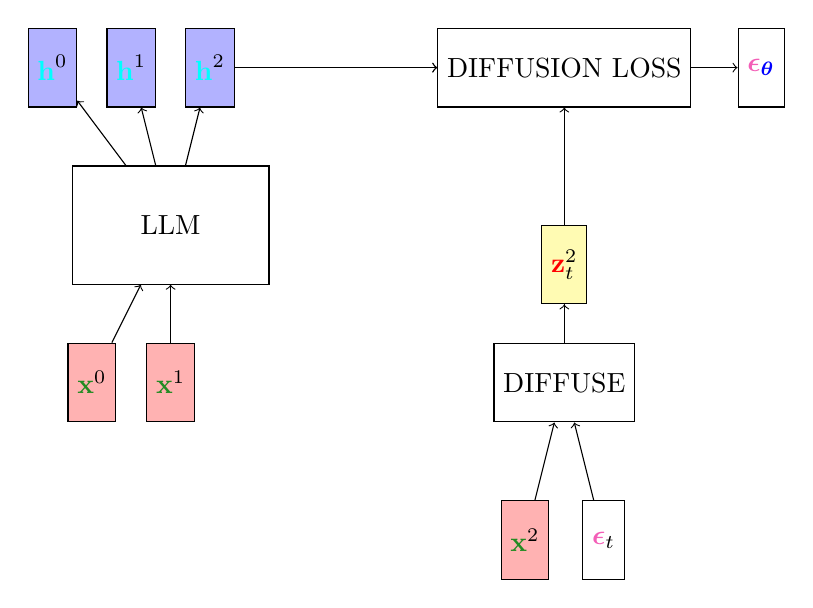
\begin{tikzpicture}
    % Nodes
    \node (LLM) at (0,0) [draw, minimum width=2.5cm, minimum height=1.5cm] {LLM};
   
    \node (h0) at (-1.5, 2) [draw, fill=blue!30, minimum height=1cm, minimum width=0.3cm] {$\vh^0$};
    \node (h1) at (-0.5, 2) [draw, fill=blue!30, minimum height=1cm, minimum width=0.3cm] {$\vh^1$};
    \node (h2) at (0.5, 2) [draw, fill=blue!30, minimum height=1cm, minimum width=0.3cm] {$\vh^2$};
   
    \node (x0) at (-1, -2) [draw, fill=red!30, minimum height=1cm, minimum width=0.3cm] {$\vx^0$};
    \node (x1) at (0, -2) [draw, fill=red!30, minimum height=1cm, minimum width=0.3cm] {$\vx^1$};

    \node (zt2) at (5, -.5) [draw, fill=yellow!30, minimum height=1cm, minimum width=0.3cm] {$\vz^2_t$};
   
    \node (diffuse) at (5, -2) [draw, minimum width=1.6cm, minimum height=1cm] {DIFFUSE};
   
    \node (diffusion_loss) at (5,2) [draw, minimum width=1.5cm, minimum height=1cm]{DIFFUSION LOSS};
   
    \node (x2) at (4.5, -4) [draw, fill=red!30, minimum height=1cm, minimum width=0.3cm] {$\vx^2$};
    \node (et) at (5.5, -4) [draw, minimum height=1cm, minimum width=0.3cm] {$\vepsilon_t$};
   
    \node (e0) at (7.5, 2) [draw, minimum height=1cm, minimum width=0.3cm] {$\vepsilon_{\vtheta}$};
   
    % Edges
    \draw[->] (x0) -- (LLM);
    \draw[->] (x1) -- (LLM);
   
    \draw[->] (LLM) -- (h0);
    \draw[->] (LLM) -- (h1);
    \draw[->] (LLM) -- (h2);
   
    \draw[->] (h2) -- (diffusion_loss);
   
    \draw[->] (h2.east) |- (diffusion_loss.west);
    \draw[->] (x2) -- (diffuse);
    \draw[->] (et) -- (diffuse);

    \draw[->] (diffuse) |- (zt2.south);
    \draw[->] (zt2) |- (diffusion_loss.south);
   
    \draw[->] (diffusion_loss.east) -- (e0);
   
\end{tikzpicture}
\caption{MAR-style architecture. The LLM consumes clean past patches $\vx^0, \vx^1$ and emits a hidden state $\vh^2$. The forward diffusion (DIFFUSE) corrupts the target patch $\vx^2$ into $\vz^2_t$ using a fresh noise sample $\vepsilon_t$. A separate diffusion head $\vepsilon_{\vtheta}$ takes $\vz^2_t$ and the LLM's hidden state $\vh^2$ as inputs. Crucially, the LLM never sees the noise: the noisy input only enters the head.}
\label{fig:llmwithdiffusion}
\end{figure}

\subsection{Approach 2: noise into the LLM (Transfusion)}

\href{https://arxiv.org/abs/2408.11039}{Transfusion} (Zhou et al., 2024) makes the opposite design choice from MAR.  Instead of keeping the noisy image latent outside the LLM and sending it to a small auxiliary denoising head, Transfusion puts the noisy image patches directly into the transformer's input sequence.  The same transformer therefore plays two roles at once: at text positions it is a normal next-token predictor, and at image positions it is a diffusion denoiser over continuous vectors.

A good way to understand the method is to separate \emph{representation}, \emph{attention}, and \emph{loss}.

\paragraph{1. Representation: one sequence, two kinds of elements.}
Text is represented as discrete tokens exactly as in a language model.  An image is first encoded into a continuous latent space, usually with a VAE, and then split into $N$ patch vectors
\[
    \vx^1,\vx^2,\ldots,\vx^N .
\]
The image patch vectors are not quantised into a codebook.  They remain real-valued vectors.  To splice an image into a text sequence, Transfusion surrounds the image block with special marker tokens:
\[
    \texttt{A cat}\;\; \texttt{<BOI>}\;\;
    \vx^1,\ldots,\vx^N\;\; \texttt{<EOI>}\;\; \texttt{is cute}.
\]
The marker tokens tell the model when it should switch from language modelling to image diffusion and back again.

\paragraph{2. Noising: corrupt the image block, not the text.}
During training, choose a diffusion time $t$ for each image and corrupt every patch in that image at the same noise level:
\begin{align}
    \vz_t^\tau
    &= \alpha_t \vx^\tau + \sigma_t \vepsilon_t^\tau,
    &
    \vepsilon_t^\tau &\sim \gauss(0,\vI),
    &
    \tau &= 1,\ldots,N .
\end{align}
The transformer input is therefore a mixed sequence: clean text token embeddings, marker-token embeddings, and noisy continuous image-patch embeddings.  A time embedding $\phi(t)$ (or equivalently a log-SNR embedding $\phi(\lambda_t)$) is added to the image-patch inputs so the transformer knows how much noise it must remove.

\paragraph{3. Attention: causal outside the image, bidirectional inside it.}
Text remains autoregressive: a text token can only attend to previous elements.  Image patches, however, have no natural left-to-right generation order, so patches within the same image block are allowed to attend to one another bidirectionally.  Across image boundaries the sequence remains causal: an image can attend to the prefix before it, and text after an image can attend to the image, but an image patch cannot attend to future text.

\paragraph{4. Loss: cross-entropy for text, diffusion MSE for images.}
The transformer output at a text position goes through the usual vocabulary head and is trained with cross-entropy.  The transformer output at an image-patch position goes through a continuous denoising head and is trained to predict the noise:
\begin{align}
    \loss_{\text{diff}}(\vtheta)
    &=
    \E\left[
        \sum_{\tau=1}^{N}
        \norm{\vepsilon_{\vtheta}^{\tau}(\vz_t^1,\ldots,\vz_t^N,t,\text{prefix})
        - \vepsilon_t^\tau}_2^2
    \right],
    \\
    \loss_{\text{Transfusion}}(\vtheta)
    &=
    \loss_{\text{LM}}(\vtheta)
    + \lambda_{\text{img}} \loss_{\text{diff}}(\vtheta).
\end{align}
The important point is that the \emph{same transformer activations} support both losses.  Only the small input/output adapters are modality-specific: text uses token embeddings and a softmax head; images use patch embeddings, time embeddings, and a continuous denoising output.

\paragraph{Inference.}
Decoding becomes a simple state machine.  In \emph{LM mode}, the model samples tokens one at a time from the softmax.  When it samples \texttt{<BOI>}, it switches to \emph{diffusion mode}: it appends $N$ pure-noise image patches $\vz_T^1,\ldots,\vz_T^N$ to the current sequence and runs the diffusion sampler.  At each denoising step, the full transformer is called on the current mixed sequence, its image-position outputs predict $\hat{\vepsilon}_t^1,\ldots,\hat{\vepsilon}_t^N$, and the sampler overwrites the image block with the next latent $\vz_{t-1}^1,\ldots,\vz_{t-1}^N$.  After the final step, the model appends \texttt{<EOI>} and switches back to LM mode.

\begin{figure}[H]
\centering
\resizebox{\textwidth}{!}{%
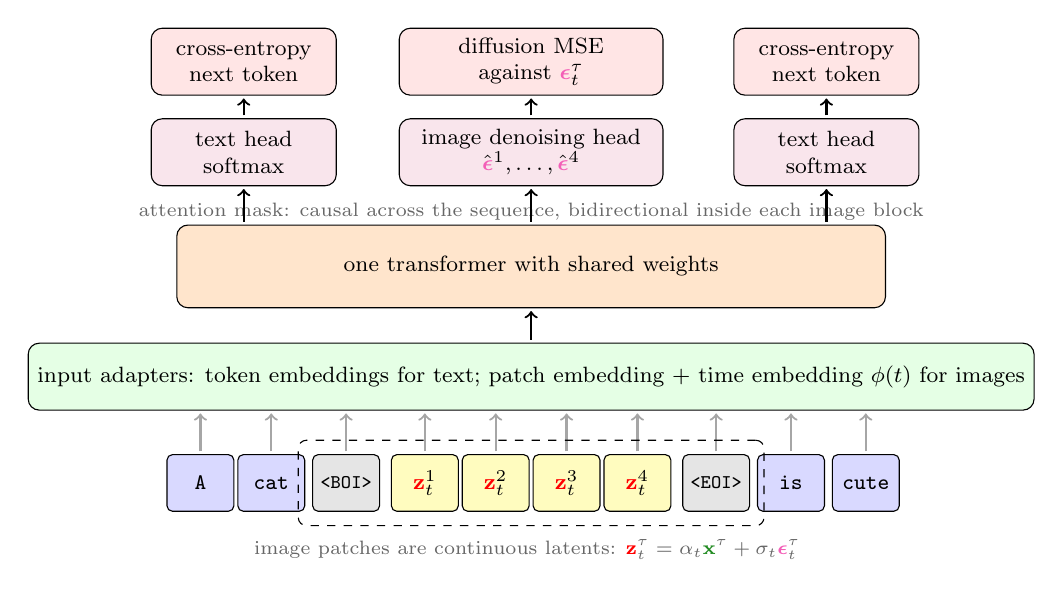
\begin{tikzpicture}[
    every node/.style={font=\small},
    tok/.style={draw, rounded corners=2pt, minimum width=0.85cm, minimum height=0.72cm,
                inner sep=1pt, font=\footnotesize},
    txt/.style={tok, fill=blue!15},
    img/.style={tok, fill=yellow!25},
    sep/.style={tok, fill=gray!20, font=\scriptsize},
    block/.style={draw, rounded corners=4pt, minimum height=0.85cm,
                  font=\footnotesize, align=center},
    adapter/.style={block, fill=green!10},
    xfmr/.style={block, fill=orange!20},
    head/.style={block, fill=purple!10},
    loss/.style={block, fill=red!10},
    note/.style={font=\scriptsize, align=center, text=gray!80!black},
    arr/.style={->, thick, shorten >=1pt, shorten <=1pt},
]
    % Input sequence.
    \node[txt] (t1)  at (0.0, 0)  {\texttt{A}};
    \node[txt] (t2)  at (0.9, 0)  {\texttt{cat}};
    \node[sep] (boi) at (1.85, 0) {\texttt{<BOI>}};
    \node[img] (p1)  at (2.85, 0) {$\vz_t^1$};
    \node[img] (p2)  at (3.75, 0) {$\vz_t^2$};
    \node[img] (p3)  at (4.65, 0) {$\vz_t^3$};
    \node[img] (p4)  at (5.55, 0) {$\vz_t^4$};
    \node[sep] (eoi) at (6.55, 0) {\texttt{<EOI>}};
    \node[txt] (t3)  at (7.50, 0) {\texttt{is}};
    \node[txt] (t4)  at (8.45, 0) {\texttt{cute}};

    \node[note] at (4.15,-0.85)
        {image patches are continuous latents: $\vz_t^\tau=\alpha_t\vx^\tau+\sigma_t\vepsilon_t^\tau$};

    % Modality-specific input adapters.
    \node[adapter, minimum width=9.0cm] (adapt) at (4.2, 1.35)
        {input adapters: token embeddings for text; patch embedding $+$ time embedding $\phi(t)$ for images};

    % Single shared transformer.
    \node[xfmr, minimum width=9.0cm, minimum height=1.05cm] (xfmr) at (4.2, 2.75)
        {one transformer with shared weights};

    \node[note] at (4.2, 3.45)
        {attention mask: causal across the sequence, bidirectional inside each image block};

    % Output heads.
    \node[head, minimum width=2.35cm] (textheadL) at (0.55, 4.2)
        {text head\\softmax};
    \node[head, minimum width=3.35cm] (imghead) at (4.20, 4.2)
        {image denoising head\\$\hat{\vepsilon}^1,\ldots,\hat{\vepsilon}^4$};
    \node[head, minimum width=2.35cm] (textheadR) at (7.95, 4.2)
        {text head\\softmax};

    % Losses.
    \node[loss, minimum width=2.35cm] (celossL) at (0.55, 5.35)
        {cross-entropy\\next token};
    \node[loss, minimum width=3.35cm] (mseloss) at (4.20, 5.35)
        {diffusion MSE\\against $\vepsilon_t^\tau$};
    \node[loss, minimum width=2.35cm] (celossR) at (7.95, 5.35)
        {cross-entropy\\next token};

    % Flow arrows.
    \foreach \n in {t1,t2,boi,p1,p2,p3,p4,eoi,t3,t4} {
        \draw[arr, gray!70] (\n.north) -- (\n.north |- adapt.south);
    }
    \draw[arr] (adapt.north) -- (xfmr.south);
    \draw[arr] (xfmr.north -| textheadL.south) -- (textheadL.south);
    \draw[arr] (xfmr.north -| imghead.south) -- (imghead.south);
    \draw[arr] (xfmr.north -| textheadR.south) -- (textheadR.south);
    \draw[arr] (textheadL.north) -- (celossL.south);
    \draw[arr] (imghead.north) -- (mseloss.south);
    \draw[arr] (textheadR.north) -- (celossR.south);

    % Image-block highlight.
    \node[draw, dashed, rounded corners=3pt, fit=(boi)(p1)(p2)(p3)(p4)(eoi),
          inner sep=5pt] {};
\end{tikzpicture}%
}
\caption{Transfusion-style training picture. Text tokens (blue), marker tokens (gray), and noisy continuous image patches (yellow) are placed into one sequence. A small set of modality-specific adapters maps them into the shared transformer space. The same transformer then feeds two kinds of output heads: a vocabulary head trained with cross-entropy at text positions, and a denoising head trained with diffusion MSE at image positions. The image block receives time conditioning and uses bidirectional attention within the block, while the mixed text-image sequence remains causal across blocks.}
\label{fig:transfusion}
\end{figure}

\subsection{Contrasting the two approaches}

Both approaches train one big transformer plus a diffusion-style MSE-on-noise loss for image patches, and both can be combined with cross-entropy on text. The differences are:

\begin{itemize}
    \item \textbf{Where the noise lives.} In MAR, the noise is contained inside a small auxiliary head and the LLM only sees clean tokens / clean past patches. In Transfusion, the noise is mixed directly into the LLM's input sequence; the LLM itself learns to denoise.
    \item \textbf{Number of forward passes per image.} MAR needs one LLM forward pass to compute $\vh^\tau$ plus, for each diffusion step, a forward pass through the diffusion head; the LLM activations can be cached. Transfusion runs the full transformer at every diffusion step, since the noisy patches change between steps. This makes Transfusion sampling more expensive per step but means the same transformer learns multi-modal representations end-to-end.
    \item \textbf{Attention pattern.} MAR uses standard causal attention end-to-end. Transfusion uses causal between-element attention with a \emph{bidirectional} window inside each image, exploiting the fact that image patches have no natural left-to-right order.
    \item \textbf{Token-versus-patch parallelism.} MAR is autoregressive over patches: patch $\tau$ is generated only after patches $1, \dots, \tau-1$. Transfusion generates all $N$ patches of an image \emph{in parallel} via diffusion, which can be substantially faster for high-resolution images.
    \item \textbf{Information bottleneck.} In MAR, everything the diffusion head knows about the past must fit through the single conditioning vector $\vh^\tau$. In Transfusion, every image-patch position attends back to the entire prefix, so the conditioning is much richer.
\end{itemize}

The Transfusion paper compares this recipe head-to-head with the alternative of \emph{quantising} images into discrete tokens and treating them like text (the Chameleon recipe). Keeping image patches continuous and using diffusion is reported to scale better and reach matching FID at less than a third of the compute. The same trade-offs we have studied throughout this tutorial therefore carry over: cross-entropy on quantised tokens is simple but throws information away, while a noise-prediction loss on continuous patches preserves it at the cost of a more elaborate sampling procedure.

A natural variant, also discussed by the Transfusion authors as future work, is to swap the diffusion loss for the flow-matching loss of the previous section, or to replace it with the $\vv$- or $\vx$-parameterised losses earlier in this tutorial. Everything we have said about schedules, parameterisations, and inference samplers applies unchanged: only the input wiring of the LLM differs.









\newpage
\section*{Appendix A: Derivation of the backward sampling Gaussian}

We need to derive the expression for the mean and variance of $q(\vz_{t} | \vz_{t+1}, \vx)$. The first step is to apply Bayes' rule:
\begin{align}
q(\vz_{t} | \vz_{t+1}, \vx)
&=
\frac{
    q(\vz_{t+1} | \vz_t, \vx)\,
    q(\vz_t | \vx)
}{
    q(\vz_{t+1} | \vx)
}
\nonumber \\
&\propto
q(\vz_{t+1} | \vz_t)\,
q(\vz_t | \vx).
\end{align}
The prior follows from the way we diffuse:
\begin{align}
q(\vz_t | \vx)
&=
\gauss(\vz_t;\alpha_t \vx, \sigma_t^2 \vI).
\end{align}
We also know that the one-step forward transition can be written as
\begin{align}
q(\vz_{t+1} | \vz_t)
&=
\gauss\!\left(
    \vz_{t+1};
    \frac{\alpha_{t+1}}{\alpha_t}\vz_t,\,
    \left(
        \sigma_{t+1}^2
        -
        \frac{\alpha_{t+1}^2}{\alpha_t^2}\sigma_t^2
    \right)\vI
\right).
\end{align}

Multiplying two Gaussians gives another Gaussian.  Define
\begin{align}
A &= \frac{\alpha_{t+1}}{\alpha_t},
&
B &= \sigma_{t+1}^2 - A^2\sigma_t^2 .
\end{align}
Here $B>0$ is the variance of the forward step from $t$ to $t+1$, assuming the log signal-to-noise ratio decreases as we add noise.  Up to constants that do not depend on $\vz_t$, the posterior is
\begin{align}
q(\vz_{t} | \vz_{t+1}, \vx)
&\propto
\exp\!\left\{
-\frac{1}{2}
\left[
    \frac{1}{B}
    \norm{\vz_{t+1}-A\vz_t}_2^2
    +
    \frac{1}{\sigma_t^2}
    \norm{\vz_t-\alpha_t\vx}_2^2
\right]
\right\}.
\end{align}

Now complete the square in $\vz_t$.  The quadratic terms give the precision
\begin{align}
\Sigma^{-1}
&=
\left(
    \frac{A^2}{B}
    +
    \frac{1}{\sigma_t^2}
\right)\vI
\nonumber \\
&=
\frac{A^2\sigma_t^2+B}{B\sigma_t^2}\vI
=
\frac{\sigma_{t+1}^2}{B\sigma_t^2}\vI,
\end{align}
where the last equality uses $A^2\sigma_t^2+B=\sigma_{t+1}^2$.  Inverting gives
\begin{align}
\Sigma
&=
\frac{B\sigma_t^2}{\sigma_{t+1}^2}\vI
\nonumber \\
&=
\left(
    \sigma_{t+1}^2
    -
    \frac{\alpha_{t+1}^2}{\alpha_t^2}\sigma_t^2
\right)
\frac{\sigma_t^2}{\sigma_{t+1}^2}\vI .
\end{align}

The linear terms give the natural-parameter vector
\[
    \frac{A}{B}\vz_{t+1}
    +
    \frac{\alpha_t}{\sigma_t^2}\vx .
\]
Therefore the mean is
\begin{align}
\vmu
&=
\Sigma
\left(
    \frac{A}{B}\vz_{t+1}
    +
    \frac{\alpha_t}{\sigma_t^2}\vx
\right)
\nonumber \\
&=
\frac{A\sigma_t^2}{\sigma_{t+1}^2}\vz_{t+1}
+
\frac{B\alpha_t}{\sigma_{t+1}^2}\vx .
\end{align}

Putting the mean and covariance together, we can write the posterior in a form that stays within the page margins:
\begin{align}
q(\vz_t|\vz_{t+1},\vx)
&=
\gauss\!\left(
    \vz_t;
    \vmu_{t|t+1},
    \Sigma_{t|t+1}
\right),
\\
\vmu_{t|t+1}
&=
\frac{\alpha_{t+1}}{\alpha_t}
\frac{\sigma_t^2}{\sigma_{t+1}^2}
\vz_{t+1}
+
\left(
    \sigma_{t+1}^2
    -
    \frac{\alpha_{t+1}^2}{\alpha_t^2}\sigma_t^2
\right)
\frac{\alpha_t}{\sigma_{t+1}^2}\vx,
\\
\Sigma_{t|t+1}
&=
\left(
    \sigma_{t+1}^2
    -
    \frac{\alpha_{t+1}^2}{\alpha_t^2}\sigma_t^2
\right)
\frac{\sigma_t^2}{\sigma_{t+1}^2}\vI .
\end{align}

It is often more convenient to express the same result in terms of the log signal-to-noise ratio
\[
    \lambda_t = \log\frac{\alpha_t^2}{\sigma_t^2}.
\]
Using
\[
    \frac{\alpha_{t+1}^2}{\sigma_{t+1}^2}
    \frac{\sigma_t^2}{\alpha_t^2}
    =
    e^{\lambda_{t+1}-\lambda_t},
\]
we obtain
\begin{align}
\vmu_{t|t+1}
&=
\frac{\alpha_t}{\alpha_{t+1}}
e^{\lambda_{t+1}-\lambda_t}
\vz_{t+1}
+
\left(
    1-e^{\lambda_{t+1}-\lambda_t}
\right)
\alpha_t\vx,
\\
\Sigma_{t|t+1}
&=
\left(
    1-e^{\lambda_{t+1}-\lambda_t}
\right)
\sigma_t^2\vI .
\end{align}
Finally, setting
\[
    c = 1-e^{\lambda_{t+1}-\lambda_t}\in(0,1),
\]
gives the compact sampler form:
\begin{align}
q(\vz_t|\vz_{t+1},\vx)
&=
\gauss\!\left(
    \vz_t;\,
    \alpha_t\left[
        \frac{1-c}{\alpha_{t+1}}\vz_{t+1}
        +
        c\vx
    \right],
    c\,\sigma_t^2\vI
\right).
\end{align}
This is the form used by the sampler.






\newpage
\section*{Appendix B}




The marginal probability distribution $p_t(\vz)$ associated with the samples generated according to our forward diffusion process
\begin{align}
\vz_t = \alpha_t \vx + \sigma_t \vepsilon_t \nonumber
\end{align}
coincides with the distribution of the probability flow ODE with velocity field:
\begin{align}
\dot{\vz}_t =  \vv(\vz, t)
\end{align}
where
\begin{align}
\vv(\vz, t) = \mathbb{E}[\dot{\vz}_t | \vz_t = \vz] = \dot{\alpha}_t \mathbb{E}[\vx | \vz_t = \vz] + \dot{\sigma}_t \mathbb{E}[\vepsilon | \vz_t = \vz].
\end{align}



The proof consists of two steps.
\begin{itemize}
\item STEP 1: Prove that $p_t(\vz)$ satisfies the transport equation
\begin{equation}
    \partial_t p_t(\vz) + \nabla_{\vz} \cdot (\vv(\vz, t) p_t(\vz)) = 0.
\end{equation}
\item STEP 2: Solve the transport equation by the method of characteristics to prove that $p_t(\vz)$ associated with the samples generated according to our forward diffusion process
\begin{align}
\vz_t = \alpha_t \vx + \sigma_t \vepsilon_t \nonumber
\end{align}
coincides with the distribution of the probability flow ODE with velocity field:
\begin{align}
\dot{\vz}_t =  \vv(\vz, t).
\end{align}
\end{itemize}

I will use the \href{https://arxiv.org/abs/2401.08740}{SiT} paper to prove STEP 1 (their Appendix A.1). I will then use ChatGPT with the following prompt to prove STEP 2.

Prompt:
\emph{Using the above statement, please prove STEP 2 in detail. Assume that I only have basic knowledge of calculus so explain all steps clearly and in detail.}







\section*{STEP 1: Derive the transport equation}

This part of the proof is from the Appendix of the \href{https://arxiv.org/abs/2401.08740}{SiT} paper. Consider the time-dependent probability density function (PDF) $p_t(\vz)$ of $\vz_t = \alpha_t \vx + \sigma_t \vepsilon$. By definition, its characteristic function $\hat{p}_t(\vk)$ is given by
\begin{equation}
    \hat{p}_t(\vk) = \mathbb{E}[e^{i \vk \cdot \vz_t}]
\end{equation}
where $\mathbb{E}$ denotes expectation over $\vx$ and $\vepsilon$. Taking time derivative on both sides, and using the tower property of conditional expectation, we have
\begin{align}
    \partial_t \hat{p}_t(\vk) &= i \vk \cdot \mathbb{E}[\dot{\vz}_t e^{i \vk \cdot \vz_t}] \label{eq:char_time_deriv_1} \\
    &= i \vk \cdot \mathbb{E}_{\rvz \sim p_t} [\mathbb{E}[\dot{\vz}_t e^{i \vk \cdot \vz_t} | \vz_t = \vz]] \label{eq:char_time_deriv_2} \\
    &= i \vk \cdot \mathbb{E}_{\rvz \sim p_t} [\mathbb{E}[(\dot{\alpha}_t \rvz_* + \dot{\sigma}_t \vepsilon) e^{i \vk \cdot \vz_t} | \vz_t = \vz]] \label{eq:char_time_deriv_3} \\
    &= i \vk \cdot \mathbb{E}_{\rvz \sim p_t} [\mathbb{E}[(\dot{\alpha}_t \rvz_* + \dot{\sigma}_t \vepsilon) | \vz_t = \vz] e^{i \vk \cdot \vz}] \label{eq:char_time_deriv_4} \\
    &= i \vk \cdot \mathbb{E}_{\rvz \sim p_t} [\vv(\vz, t) e^{i \vk \cdot \vz}] \label{eq:char_time_deriv_5}
\end{align}
where $\vv(\vz, t) = \mathbb{E}[(\dot{\alpha}_t \rvz_* + \dot{\sigma}_t \vepsilon) | \vz_t = \vz] = \dot{\alpha}_t \mathbb{E}[\rvz_* | \vz_t = \vz] + \dot{\sigma}_t \mathbb{E}[\vepsilon | \vz_t = \vz]$ is the velocity defined in Eq. (3). Explicitly, Eq. \eqref{eq:char_time_deriv_5} reads
\begin{equation}
    \partial_t \int_{\mathbb{R}^d} e^{i \vk \cdot \vz} p_t(\vz) d\vz = i \vk \cdot \int_{\mathbb{R}^d} \vv(\vz, t) e^{i \vk \cdot \vz} p_t(\vz) d\vz
\end{equation}
from which we deduce
\begin{align}
    \int_{\mathbb{R}^d} e^{i \vk \cdot \vz} \partial_t p_t(\vz) d\vz &= \int_{\mathbb{R}^d} \vv(\vz, t) \cdot \nabla_{\vz} [e^{i \vk \cdot \vz}] p_t(\vz) d\vz \\
    &= -\int_{\mathbb{R}^d} \nabla_{\vz} \cdot [\vv(\vz, t) p_t(\vz)] e^{i \vk \cdot \vz} d\vz
\end{align}
where $\nabla_{\vz} \cdot [\vv p_t] = \sum_{i=1}^{d} \frac{\partial}{\partial z_i} [v_i p_t]$ is the divergence operator and we used integration by parts to get the second equality. By the properties of the Fourier transform, uniqueness for all frequencies, the last equation implies that $p_t(\vz)$ satisfies the transport equation (a partial differential equation for $p$ in terms of $t$ and $\vz$):
\begin{equation}
    \partial_t p_t(\vz) + \nabla_{\vz} \cdot (\vv(\vz, t) p_t(\vz)) = 0.
\end{equation}
Solving this equation by the method of characteristics leads to probability flow ODE, as shown by ChatGPT in the following section.


\section*{STEP 2: Solution by method of characteristics}

We wish to prove that the marginal probability density
\[
p_t(\vz)
\]
of the forward diffusion process
\[
\vz_t = \alpha_t \vx + \sigma_t \vepsilon_t,
\]
which satisfies the transport equation
\[
\partial_t p_t(\vz) + \nabla_{\vz} \cdot \Bigl( \vv(\vz,t) \, p_t(\vz) \Bigr) = 0,
\]
with the velocity field
\[
\vv(\vz,t) = \dot{\alpha}_t \, \mathbb{E}[\vx \mid \vz_t = \vz] + \dot{\sigma}_t \, \mathbb{E}[\vepsilon \mid \vz_t = \vz],
\]
is equivalent to the density obtained by solving the probability flow ODE
\[
\dot{\vz}_t = \vv(\vz,t).
\]

\subsection*{Part A: Expanding the Transport Equation}

First, we rewrite the transport equation:
\[
\partial_t p_t(\vz) + \nabla_{\vz} \cdot \Bigl( \vv(\vz,t) \, p_t(\vz) \Bigr) = 0.
\]
Expanding the divergence term by the product rule gives
\[
\nabla_{\vz} \cdot \Bigl( \vv(\vz,t) \, p_t(\vz) \Bigr) = \vv(\vz,t) \cdot \nabla_{\vz} p_t(\vz) + p_t(\vz) \, \nabla_{\vz} \cdot \vv(\vz,t).
\]
Thus, the transport equation becomes
\[
\partial_t p_t(\vz) + \vv(\vz,t) \cdot \nabla_{\vz} p_t(\vz) + p_t(\vz) \, \nabla_{\vz} \cdot \vv(\vz,t) = 0.
\]

\subsection*{Part B: Introducing the Characteristic Curves}

The method of characteristics reduces the PDE to an ODE along paths (or \emph{characteristics}) defined by
\[
\frac{d\vz(t)}{dt} = \vv\bigl(\vz(t), t\bigr).
\]
For any starting point \(\vz_{t_0}\) at time \(t_0\) (for example, at \(t=T\) where the density is known), we denote the trajectory by
\[
\vz(t) = \phi_{t,t_0}(\vz_{t_0}).
\]

\subsection*{Part C: Computing the Total Derivative Along a Characteristic}

Consider $p_t\bigl(\vz(t)\bigr)$,
which is the density along the trajectory. By the chain rule,
\[
\frac{d}{dt} p_t\bigl(\vz(t)\bigr) = \partial_t p_t\bigl(\vz(t)\bigr) + \frac{d\vz(t)}{dt} \cdot \nabla_{\vz} p_t\bigl(\vz(t)\bigr).
\]
Since \(\frac{d\vz(t)}{dt} = \vv\bigl(\vz(t),t\bigr)\), we obtain
\[
\frac{d}{dt} p_t\bigl(\vz(t)\bigr) = \partial_t p_t\bigl(\vz(t)\bigr) + \vv\bigl(\vz(t),t\bigr) \cdot \nabla_{\vz} p_t\bigl(\vz(t)\bigr).
\]
Comparing this with our expanded transport equation at the point \(\vz(t)\),
\[
\partial_t p_t\bigl(\vz(t)\bigr) + \vv\bigl(\vz(t),t\bigr) \cdot \nabla_{\vz} p_t\bigl(\vz(t)\bigr) = - p_t\bigl(\vz(t)\bigr) \, \nabla_{\vz} \cdot \vv\bigl(\vz(t),t\bigr),
\]
we find that along a characteristic,
\[
\frac{d}{dt} p_t\bigl(\vz(t)\bigr) = - p_t\bigl(\vz(t)\bigr) \, \nabla_{\vz} \cdot \vv\bigl(\vz(t),t\bigr).
\]

\subsection*{Part D: Solving the ODE for the Density}

The ODE
\[
\frac{d}{dt} p_t\bigl(\vz(t)\bigr) = - p_t\bigl(\vz(t)\bigr) \, \nabla_{\vz} \cdot \vv\bigl(\vz(t),t\bigr)
\]
is separable. We rewrite it as
\[
\frac{1}{p_t\bigl(\vz(t)\bigr)} \frac{d}{dt} p_t\bigl(\vz(t)\bigr) = - \nabla_{\vz} \cdot \vv\bigl(\vz(t),t\bigr).
\]
Integrate both sides from an initial time \(t_0\) (e.g., \(T\)) to time \(t\):
\[
\int_{t_0}^{t} \frac{1}{p_s\bigl(\vz(s)\bigr)} \frac{d}{ds} p_s\bigl(\vz(s)\bigr) \, ds
= - \int_{t_0}^{t} \nabla_{\vz} \cdot \vv\bigl(\vz(s),s\bigr) \, ds.
\]
The left-hand side integrates to
\[
\ln p_t\bigl(\vz(t)\bigr) - \ln p_{t_0}\bigl(\vz(t_0)\bigr) = \ln\!\left( \frac{p_t\bigl(\vz(t)\bigr)}{p_{t_0}\bigl(\vz(t_0)\bigr)} \right).
\]
Thus, we have
\[
\ln\!\left( \frac{p_t\bigl(\vz(t)\bigr)}{p_{t_0}\bigl(\vz(t_0)\bigr)} \right)
= - \int_{t_0}^{t} \nabla_{\vz} \cdot \vv\bigl(\vz(s),s\bigr) \, ds,
\]
and exponentiating both sides yields
\[
p_t\bigl(\vz(t)\bigr) = p_{t_0}\bigl(\vz(t_0)\bigr) \exp\!\left(- \int_{t_0}^{t} \nabla_{\vz} \cdot \vv\bigl(\vz(s),s\bigr) \, ds\right).
\]

\subsection*{Part E: Interpreting the Result as a Change of Variables}

The above expression shows how the density changes along the flow. In fact, if we consider the change of variables induced by the mapping
\[
\vz(t) = \phi_{t,t_0}(\vz(t_0)),
\]
the density transforms as
\[
p_t(\vz) = p_{t_0}(\vz_0) \left|\det \frac{\partial \vz(t)}{\partial \vz_0}\right|^{-1}.
\]
It turns out that the derivative of the log-determinant of the Jacobian matrix satisfies
\[
\frac{d}{dt} \ln \left|\det \frac{\partial \vz(t)}{\partial \vz_0}\right|
= \nabla_{\vz} \cdot \vv\bigl(\vz(t),t\bigr).
\]
Thus, the exponential factor in our solution exactly accounts for the change in volume (i.e., the local expansion or contraction) induced by the flow.

\subsection*{Part F: Concluding the Proof}

Since the forward diffusion process is defined by
\[
\vz_t = \alpha_t \vx + \sigma_t \vepsilon_t,
\]
its marginal density is given by
\[
p_t(\vz) = \int p(\vx) \, \mathcal{N}\Bigl(\vz; \alpha_t \vx,\, \sigma_t^2 \vI\Bigr) \, d\vx.
\]
At the final time \(T\), we typically have
\[
\vz_T = \alpha_T \vx + \sigma_T \vepsilon_T,
\]
with \(\vepsilon_T\) chosen so that \(p_T(\vz)\) is a simple distribution (often a standard Gaussian).

By solving the probability flow ODE backward in time from \(\vz_T \sim \mathcal{N}(\vzero, \vI)\), the density evolves as
\[
p_t\bigl(\vz(t)\bigr) = p_T\bigl(\vz(T)\bigr) \exp\!\left(- \int_{T}^{t} \nabla_{\vz} \cdot \vv\bigl(\vz(s),s\bigr) \, ds\right).
\]
Since this evolution is unique given the initial condition at \(T\), the density obtained by \emph{pushing forward} the Gaussian through the probability flow ODE exactly matches the marginal density obtained from the forward diffusion process.
This completes the detailed proof of STEP 2.

\end{document}